\documentclass[xcolor=x11names]{beamer}
%%%%%%%%%%%%%%%%%%%%%%%%%%%%%%%%%%%%%%%%%%%%%%%%%%%%%%%%%%%%
%%  This Beamer template was created by Cameron Bracken.
%%  Anyone can freely use or modify it for any purpose
%%  without attribution.
%%
%%  Last Modified by C. Bracken: January 9, 2009
%%
%%  The preamble, and maybe some modification of the Cameron Bracken's template is due to Attila Molnár.
%%
%%

%% General document
\usepackage[utf8]{inputenc}
\usepackage[T1]{fontenc}
\usepackage{graphicx}
\usepackage{tikz}
\usetikzlibrary{decorations.fractals}
\usetikzlibrary{decorations.text}
\usepgflibrary{arrows}
\usetikzlibrary{fadings}
\usetikzlibrary[decorations.pathmorphing]
\tikzfading[name=fade inside, inner color=transparent!70, outer color=transparent!70]
\usetikzlibrary{calc}
\usetikzlibrary{intersections}
\usetikzlibrary{shapes}
\usetikzlibrary{patterns}
\usefonttheme{serif}
\usepackage{amssymb} 			
\usepackage{amsmath}
\usepackage{ifthen}
\usepackage[normalem]{ulem}
\usepackage{mathrsfs}

%%%%%%%%%%%%%%%%%%%%%%%%%%%%%%%%%%%%%%%%%%%%%%%%%%%%%%%%%%%%%%%%%%%%%%%%%%%%%%%%%%%%
%% Beamer Layout %%%%%%%%%%%%%%%%%%%%%%%%%%%%%%%%%%
\useoutertheme[subsection=false,shadow]{miniframes}
\useinnertheme{default}
\usefonttheme{serif}
%\usepackage{txfonts} %Hook for strict implication!
\DeclareSymbolFont{symbolsC}{U}{txsyc}{m}{n}
\DeclareMathSymbol{\strictif}{\mathrel}{symbolsC}{74}
\DeclareMathSymbol{\boxright}{\mathrel}{symbolsC}{128}
\usepackage{palatino}
%\usepackage[uppercase=upright,charter]{mathdesign}

\setbeamerfont{title like}{shape=\scshape}
\setbeamerfont{frametitle}{shape=\scshape}


\setbeamercolor*{lower separation line head}{bg=white!40!DeepSkyBlue3}
\setbeamercolor*{normal text}{fg=black,bg=white}
\setbeamercolor*{alerted text}{fg=red}
\setbeamercolor*{example text}{fg=black}
\setbeamercolor*{structure}{fg=black}

\setbeamercolor*{palette tertiary}{fg=black,bg=white!90!DeepSkyBlue3}
\setbeamercolor*{palette quaternary}{fg=black,bg=black!10}

%\setbeamercolor{block body alerted}{bg=normal text.bg!90!DeepSkyBlue4}
\setbeamercolor{block body}{bg=normal text.bg!95!DeepSkyBlue3}
%\setbeamercolor{block body example}{bg=normal text.bg!90!DeepSkyBlue4}
%\setbeamercolor{block title alerted}{use={normal text,alerted text},fg=alerted text.fg!75!normal text.fg,bg=normal text.bg!90!DeepSkyBlue4}
\setbeamercolor{block title}{bg=normal text.bg!70!DeepSkyBlue3}
%\setbeamercolor{block title example}{use={normal text,example text},fg=example text.fg!75!normal text.fg,bg=normal text.bg!75!DeepSkyBlue4}

\setbeamertemplate{blocks}[rounded][shadow=true]
%\setbeamertemplate{background canvas}[vertical shading][bottom=white,top=structure.fg!25]
%\setbeamertemplate{sidebar canvas left}[horizontal shading][left=white!40!black,right=black]
\setbeamertemplate{itemize items}[circle]
\setbeamercolor*{itemize item}{fg=DeepSkyBlue3}
\setbeamercolor*{itemize subitem}{fg=DeepSkyBlue3}
\setbeamercolor*{itemize subsubitem}{fg=DeepSkyBlue3}
\setbeamertemplate{enumerate items}[circle]
%\setbeamercolor{item projected}{bg=DeepSkyBlue3,fg=black}
\setbeamercolor{item projected}{bg=white,fg=DeepSkyBlue3}
\setbeamercolor*{enumerate item}{fg=DeepSkyBlue3}
\setbeamercolor*{enumerate subitem}{fg=DeepSkyBlue3}
\setbeamercolor*{enumerate subsubitem}{fg=DeepSkyBlue3}

%%%%%%%%%%%%%%%%%%%%%%%%%%%%%%%%%%%%%%%%%%%%%%%%%%


%%%%%%%%%%%%%%%%%%%%%%%%%%%%%%%%%%%%%%%%%%%%%%%%%%%%%%%%%%%%%%%%%%%%%%%%%%%%%%%%%%%%

\newenvironment{defi}[1][]{\begin{block}{\footnotesize \textsc{Definition} \ifthenelse{\equal{#1}{}}{}{\, (#1)}}}{\end{block}}
\newenvironment{prop}[1][]{\begin{block}{\footnotesize \textsc{Proposition} \ifthenelse{\equal{#1}{}}{}{\, (\textsc{#1})}}}{\end{block}}
\newenvironment{lemm}[1][]{\begin{block}{\footnotesize \textsc{Lemma} \ifthenelse{\equal{#1}{}}{}{\, (\textsc{#1})}}}{\end{block}}
\newenvironment{idea}[1][]{\begin{block}{\footnotesize \textsc{Idea} \ifthenelse{\equal{#1}{}}{}{\, (\textsc{#1})}}}{\end{block}}
\newenvironment{rema}[1][]{\begin{block}{\footnotesize \textsc{Remark} \ifthenelse{\equal{#1}{}}{}{\, (\textsc{#1})}}}{\end{block}}
\newenvironment{coro}[1][]{\begin{block}{\footnotesize \textsc{Corollary} \ifthenelse{\equal{#1}{}}{}{\, (\textsc{#1})}}}{\end{block}}
\newenvironment{tete}[1][]{\begin{block}{\footnotesize \textsc{Theorem} \ifthenelse{\equal{#1}{}}{}{\, (\textsc{#1})}}}{\end{block}}
\newenvironment{claim}[1][]{\begin{block}{Claim \ifthenelse{\equal{#1}{}}{}{\, (\textsc{#1})}}}{\end{block}}
%\newenvironment{lemma}[1][]{\begin{block}{Lemma \ifthenelse{\equal{#1}{}}{}{\, (\textsc{#1})}}}{\end{block}}
\newenvironment{question}[1][]{\begin{block}{Question \ifthenelse{\equal{#1}{}}{}{\, (\textsc{#1})}}}{\end{block}}
\newenvironment{rem}[1][]{\begin{block}{Remark \ifthenelse{\equal{#1}{}}{}{\, (\textsc{#1})}}}{\end{block}}
\newenvironment{homework}[1][]{\begin{block}{Homework \ifthenelse{\equal{#1}{}}{}{\, (\textsc{#1})}}}{\end{block}}
\newenvironment{proo}[1][]{\begin{block}{\footnotesize \textsc{Proof} \ifthenelse{\equal{#1}{}}{}{\, (\textsc{#1})}}}{\end{block}}

%%%%%%%%%%%%%%%%%%%%%
%% To evade unnecessary circles, mainly for \cimdia
%%%%%%%%%%%%%%%%%%%%%

\makeatletter
\let\beamer@writeslidentry@miniframeson=\beamer@writeslidentry
\def\beamer@writeslidentry@miniframesoff{%
  \expandafter\beamer@ifempty\expandafter{\beamer@framestartpage}{}% does not happen normally
  {%else
    % removed \addtocontents commands
    \clearpage\beamer@notesactions%
  }
}
\newcommand*{\miniframeson}{\let\beamer@writeslidentry=\beamer@writeslidentry@miniframeson}
\newcommand*{\miniframesoff}{\let\beamer@writeslidentry=\beamer@writeslidentry@miniframesoff}
\makeatother

%%%%%%%%%%%%%%%%%%%%%%%%%%%%%
%%%%%%%%%%%%% END %%%%%%%%%%%
%%%%%%%%%%%%%%%%%%%%%%%%%%%%%


%%%% Formatting Commands

\newcommand{\cimdia}[1] {\miniframesoff \begin{frame}\begin{center}\huge \begin{tabular}{c}#1\end{tabular}\end{center}\end{frame}\miniframeson}
\newcommand{\szakasz}[2][]{\section{#1}\subsection{}\cimdia{#2}}
\newcommand{\bluebullet}{\textcolor{DeepSkyBlue3}{\quad $\bullet$} \,\,}

\newenvironment{frame*}[1][]{\miniframesoff \begin{frame} #1}{\end{frame}\miniframeson}

  % for admissible intersections
  \newcommand{\bigsqcap}{\rotatebox[origin=c]{180}{$\bigsqcup$}}

  % Intelligent curves for tikz:
  % Use it in this way: \gorbe{elejenev}{vegenev}{elejeszog}{elejelendulet}{vegeszog}{vegelendulet};
  \newcommand{\gorbe}[6]{\draw (#1).. controls ([shift=(#3: #4 cm)]#1) and ([shift=(#5: #6 cm)]#2) .. (#2);}
  \newcommand{\gorbefelirattal}[8]{\draw (#1).. controls ([shift=(#3: #4 cm)]#1) and ([shift=(#5: #6 cm)]#2) .. (#2) node[#8] {#7};}

\newcommand{\pipa}{%
\begin{tikzpicture}[green!50!black, thick, scale=.1]
\gorbe{0,1}{2,2}{-80}{1}{225}{.7}
\end{tikzpicture}}

\newcommand{\ellentmondas}
		{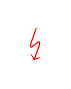
\begin{tikzpicture}[scale=0.2]
			\draw[rounded corners=3pt, rotate=10, red,
					->] (0.75,2)--(0,0.66)--(1,1.33)--(0.25,0);
		\end{tikzpicture}}
\newcommand{\indirektfelteves}
		{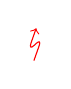
\begin{tikzpicture}[scale=0.2]
			\draw[rounded corners=3pt, rotate=10, red,
					<-] (0.75,2)--(0,0.66)--(1,1.33)--(0.25,0);
		\end{tikzpicture}}

\newcommand{\pecset}[2]{\begin{tikzpicture}[remember picture,overlay]
\node [ draw=red,
        rectangle,
        rounded corners=5mm,
        inner sep=1mm,
        ultra thick,
        fill=white,
        fill opacity=.8,
        rotate=30,
        scale=#1,
        text opacity=0.7]
        at (current page.center)
        {#2};
\end{tikzpicture}}

%\felirat{inner sep}{rounded corners}{scale}{x}{y}{text}
\newcommand{\felirat}[7][]{\begin{tikzpicture}[remember picture,overlay]
\node [draw=DeepSkyBlue3, rectangle, rounded corners=#3 mm, inner sep=#2mm, ultra thick, fill=white, fill opacity=.8, scale=#4, text opacity=1,#1]
at ([xshift=#5 cm, yshift=#6 cm]current page.center) {#7};
\end{tikzpicture}}

\newcommand{\hazi}[6]{\begin{tikzpicture}[remember picture,overlay]
\node [ draw=Coral1,
        rectangle,
        rounded corners=#2 mm,
        inner sep=#1mm,
        ultra thick,
        fill=white,
        fill opacity=.8,
        rotate=0,
        scale=#3,
        text opacity=1]
        at ([xshift=#4 cm, yshift=#5 cm]current page.center)
        {#6};
\end{tikzpicture}}


% Emphasizing:
\definecolor{barna}{rgb}{0.5,0.2,0.1}
\newcommand{\bemph}[1] {{\color{DeepSkyBlue3}{#1}}}
\newcommand{\kemph}[1] {{\color{blue}{#1}}}
\newcommand{\cemph}[1]{\textcolor{red}{#1}}
\newcommand{\zemph}[1] {{\color{Green2}{#1}}}
\newcommand{\yemph}[1] {{\color{Orange1}{#1}}}
\renewcommand{\emph}[1]{\textbf{#1}}

\newcommand{\FD}{\mathbf F}
\newcommand{\FB}{\mathbf G}
\newcommand{\PD}{\mathbf P}
\newcommand{\PB}{\mathbf H}

\newcommand{\FDDot}{\underline{\mathbf F}}
\newcommand{\FBDot}{\underline{\mathbf G}}
\newcommand{\PDDot}{\underline{\mathbf P}}
\newcommand{\PBDot}{\underline{\mathbf H}}


% i dont know whats this
\newcommand{\matbuborek}[1]{%
\begin{tikzpicture}
\node[draw=black, rounded corners=2pt, rectangle, inner sep=1mm] at (0,0){$#1$};
\end{tikzpicture}}


\newcommand{\dzsa}[1]{\textsc{\underline{#1}}:}

% modal operators:
 \newcommand{\diamondmeret}{.18}
 \newcommand{\boxmeret}{4*\diamondmeret/5}


 \newcommand{\mland} [1][.1]{\hspace{#1cm}\textup{and}\hspace{#1cm}}
 \newcommand{\mlthen}[1][.1]{\hspace{#1cm}\Rightarrow\hspace{#1cm}}
 \newcommand{\mlnot} [1][.1]{\hspace{#1cm}\textup{not }}
 \newcommand{\mlor}  [1][.1]{\hspace{#1cm}\textup{or}\hspace{#1cm}}
 \newcommand{\mliff} [1][.1]{\hspace{#1cm}\mliff\hspace{#1cm}}
 \newcommand{\vonal} [1][.2]{\hspace{#1cm} | \hspace{#1cm}}
 \newcommand{\mlwhere} [1][.2]{\hspace{#1cm}\textup{where}\hspace{#1cm}}
 \newcommand{\lrule}[3][c]{\begin{array}{#1} #2  \\  \hline #3 \end{array}}
 \newcommand{\dlrule}[3][c]{\begin{array}{#1} #2  \\  \hline\hline #3 \end{array}}
 \newcommand{\dual}{\delta}
\newcommand{\Dajmond}{\lozenge}
\newcommand{\Boksz}{\square}
\newcommand{\felDajmond}{\blacklozenge}
\newcommand{\felBoksz}{\blacksquare}
\newcommand{\felle}	
	{\,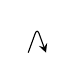
\begin{tikzpicture}
		\pgfmathsetmacro{\szog}{70}
		\pgfmathsetmacro{\hossz}{0.33}
	\draw[->,>=stealth,rounded corners=2pt] (0,0)	--(\szog:\hossz cm)
								--([shift=(-\szog :\hossz cm)]\szog:\hossz cm);	
	\end{tikzpicture}\,}
\newcommand{\lefel}
	{\, 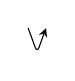
\begin{tikzpicture}
		\pgfmathsetmacro{\szog}{70}
		\pgfmathsetmacro{\hossz}{0.33}
		\draw[->,>=stealth,rounded corners=2pt] (0,0)	--(-\szog:\hossz cm)
								--([shift=(\szog :\hossz cm)]-\szog:\hossz cm);
	\end{tikzpicture}\, }
\newcommand{\enn}
{\mathbf{N}}
\newcommand{\nne}
{\reflectbox{$\mathbf{N}$}}

\newcommand{\mono}{\rightarrowtail}
\newcommand{\epi}{\twoheadrightarrow}
\newcommand{\iso}{\rightarrowtail \!\!\!\!\! \rightarrow}

 \newcommand{\defegy}[1][.1]{\hspace{#1cm}\overset{\textup{\tiny def}}{=}\hspace{#1cm}}
 \newcommand{\defpont}[1][.1]{\hspace{#1cm}\overset{\textup{\tiny def}}{:}\hspace{#1cm}}
 \newcommand{\defekv}[1][.1]{\hspace{#1cm}\overset{\textup{\tiny def}}{ \Leftrightarrow }\hspace{#1cm}}
 \newcommand{\lthen}{\rightarrow}
 \newcommand{\liff}{\leftrightarrow}
 \newcommand{\lminus}{-}
 \newcommand{\lsup}{\mbox{$\mathop{\sim}$}}
 \newcommand{\colnot}{\mbox{$\mathop{\sim}$}}
 \newcommand{\forallin}[2]{(\forall #1 \in #2)}
 \newcommand{\existsin}[2]{(\exists #1 \in #2)}
 \newcommand{\nexistsin}[2]{(\nexists #1 \in #2)}
 \newcommand{\forallp}[1]{(\forall #1)}
 \newcommand{\existsp}[1]{(\exists #1)}
 \newcommand{\forallR}[2]{(\forall #1 \reflectbox{$R$} #2)}
 \newcommand{\existsR}[2]{(\exists #1 \reflectbox{$R$} #2)}
\newcommand{\magyarazat}[2]{\overset{\substack{\textup{#2}\\ \downarrow}}{#1}}
\newcommand{\magyi}[1]{\textup{\bemph{\tiny #1}}}


\newcommand{\bintension}[2][]{{{[}\!{[}} {#2}{{]}\!{]}}^{\mathcal{#1}}}
\newcommand{\wintension}[3][]{{[}\hspace{-.46mm}{[} {#3}{]}\hspace{-.46mm}{]}^{\mathfrak{#1}}_{#2}}
\newcommand{\canintension}[2][]{{[}\hspace{-.46mm}{[} {#2}{]}\hspace{-.46mm}{]}_{\mathrm{#1}}}
\newcommand{\jelentes}[2]{{{[}\!{[}} {#1}{{]}\!{]}}^{{#2}}}
\newcommand{\intension}[2][]{{[}\hspace{-.46mm}{[} {#2}{]}\hspace{-.46mm}{]}^{\mathfrak{#1}}}
\newcommand{\Kintension}[2][]{|\!| {#2} |\!|^{\mathcal{#1}}}
\newcommand{\theory}[2][]{\mathrm{th}_{\mathfrak{#1}}(#2)}
\newcommand{\seenby}{\reflectbox {$R$}}
\newcommand{\derives}[1][]{\vdash_{\mathrm{#1}}}
\newcommand{\ugyanaz}[1]{\mathrel{\overset{#1}{\equiv}}}


\newcommand{\harmasosztas}[6]{

\begin{minipage}{#1\textwidth}%
#4%
\end{minipage}%
\begin{minipage}{#2\textwidth}%
#5%
\end{minipage}%
\begin{minipage}{#3\textwidth}%
#6%
\end{minipage}

}


\newcommand{\felkor}[8]{%
\begin{scope}[draw=#5,very thick,fill opacity=.15,draw opacity=.5,text opacity=1]
\draw[fill=#5]
([shift=(#3:#2)]#1) arc (#3:180+#3:#2) -- cycle;
\node at ([shift=(#7*180+#3:#2),shift=(-#7*90+135+#3:0.5*#6)]#1){#8};
\clip ([shift=(#3:#2)]#1) arc (#3:180+#3:#2);
 \draw[fill=#5] ([shift=(#7*180+#3:#2)]#1) circle (#6);
\end{scope}
}
\newcommand{\felkorvonal}[2]{
\draw[rounded corners=0] (180+#1:.25*#2 cm) arc (180+#1:360+#1:.25*#2 cm)--cycle;
}


\newcommand{\BoxTemplate}[1]{{#1} \mathop{\Box\hspace{-1.35ex} \raisebox{.5ex}{\scalebox{.5}{$\lthen$}}}}
\newcommand{\DiamondTemplate}[1]{#1\hspace{-.2ex} \mathop{\Diamond\hspace{-1.35ex} \raisebox{.4ex}{\scalebox{.5}{$\land$}}}\,}

%%%%%%%%%%%%%%%%%%%%%%%%%%%%%%%%%%%%%%%%%%%%%%%%%%%%%%
\newenvironment{tomb}[2][.1]{\arraycolsep=#1cm\begin{array}{#2}}{\end{array}}
\beamertemplatenavigationsymbolsempty


\author{Attila Moln\'ar}
\date{2014. March 21.}
\title{Axiomatization of Kripkean FOML}
\institute{ELTE}
\begin{document}
\footnotesize


\begin{frame}
\centering
\textsc{\Large Relativistic Temporal Logic \\[1em] Definability and Completeness}

\bigskip

{ \small Attila Moln\'ar

    \textit{E\"otv\"os Lor\'and University}}

 \begin{figure}

\includegraphics[scale=.3]{elte_cimer.png}
 \end{figure}

	\today
\end{frame}

%%%%%%%%%%%%%%%%%%%%%%%%%%%%%%%%%%%%%%%%%%%%%%%%%%%%%%%%%%%%%%%%%%%%%%%%%%%%%%%%%%%%%%%%%%%%%%%%%%%5
%%%%%%%%%%%%%%%%%%%%%%%%%%%%%%%%%%%%%%%%%%%%%%%%%%%%%%%%%%%%%%%%%%%%%%%%%%%%%%%%%%%%%%%%%%%%%%%%%%%5

\szakasz[Definability]{Definability}

\begin{frame}
	\frametitle{Models}
\footnotesize

A \emph{model} $\mathfrak M $ is a pair $\langle \mathfrak F, V\rangle$ where
\begin{itemize}
\item $\mathfrak F$ is a frame $\mathfrak F=\langle W, R\rangle$,
\item $V$ is an evaluation $V: \textup{At}\to \mathcal P(W)$.
\end{itemize}
We define the \emph{satisfaction} or \emph{local truth} relation in the following way:

\[\begin{array}{lcl}
   \mathfrak M , w \models p &\defekv & w\in V(p)
\\ \mathfrak M , w \models \lnot \varphi &\defekv & \textup{ it is not true that }\mathfrak M , w \models \varphi
\\ \mathfrak M , w \models \varphi \land \psi &\defekv & \mathfrak M , w \models \varphi\textup{ and }\mathfrak M , w \models \psi
\\ \mathfrak M , w \models \FD \varphi &\defekv & \exists v \big( w<v \land \mathfrak M , v \models \varphi\big)
\\ \mathfrak M , w \models \PD \varphi &\defekv & \exists v \big( v<w \land \mathfrak M , v \models \varphi\big)
\end{array}\]

We define the \emph{global truth} or just simply the \emph{truth} relation based on the local truth:

\[ \mathfrak M \models \varphi \iff \forall w \; \mathfrak M, w \models \varphi \]

And the most important: we say that $\varphi$ is valid of $\mathfrak F$ iff it is true \textit{no matter what are the meanings of its atomic particles}:
\[ \mathfrak F \models \varphi \iff \forall V \; \mathfrak F, V \models \varphi \]

\felirat{1.5}{1}{.6}{4.2}{-4}{ \begin{minipage}{6.5cm}
Why is the latter so important? Because only the structure matters here. So by investigating validities, we will able to investigate the structure of time, while we keep the local perspective of the modal language.
\end{minipage}}
\hazi{2}{1}{.7}{3}{3.2}{\begin{tabular}{l}Give a countermodel \\ a) for every formula what we labelled `strange', such that  \\ b) for some formula what we labelled `fine'. \\ (\bemph{i.e., give a model in which the formula in question is not true} \\ \bemph{(i.e., false in some world of it)})\end{tabular}}
\end{frame}

%%%%%%%%%%%%%%%%%%%%%%%%%%%%%%%%%%%%%%%%%%%%%%%%%%%%%%%%%%%%%%%%%%%%%%%%%%%%%%%%%%%%%%%%%%%%%%%%%%%5


\begin{frame}
%\frametitle{A-B Correspondences (modal definability)}
\vspace{-.2cm}
\begin{center}A-B Correspondences (modal definability)\end{center}
\vspace{-.2cm}
\scriptsize
\[\hspace{-.9cm}\begin{array}{cclll}
\rotatebox{0}{\textup{\tiny Difficulty}} & \textup{\tiny Name} & \textup{\tiny TL formula} & \textup{\tiny FOL formula} &\textup{\tiny Name}
\\ \hline
\\[-.7em]  \textup{\tiny Easy}& \textbf {T} & \Box \varphi \lthen \varphi & \forall w \; wRw &\textup{\tiny reflexive}
\\ \textup{\tiny Easy}& \textbf {4} & \Box \varphi \lthen \Box\Box\varphi & \forall {wvu}.\; wRvRu\lthen wRu &\textup{\tiny transitive}
\\ \textup{\tiny Normal}& \textbf {Den} & \Box \Box \varphi \lthen \Box \varphi &\forall {wv} . \; wRu\lthen \existsp v wRvRu &\textup{\tiny dense}
\\ \textup{\tiny Easy}& \textbf {B} & \varphi \lthen \Box \Diamond\varphi &\forall {wv} .\;wRv\lthen vRw &\textup{\tiny symmetric}
\\ \textup{\tiny Normal}& \textbf {E} & \Diamond \varphi \lthen \Box \Diamond\varphi &\forall {wv} .\;u\reflectbox{$R$}wRv\lthen vRu &\textup{\tiny euclidean}
\\ \textup{\tiny Normal}& \textbf {G} & \Diamond \Box \varphi \lthen \Box \Diamond\varphi &\forall {wvu}.\;v\reflectbox {$R$}wRu\lthen  \existsp{u'} (vRu'\reflectbox {$R$}u) &\textup{\tiny convergent}
\\ \textup{\tiny Normal}& \textbf {.3} & \Diamond \varphi \land \Diamond \psi \lthen &\forall {wvu}.\;v\reflectbox {$R$}wRu\lthen (vRu \lor v\reflectbox {$R$}u \lor u=v) &\textup{\tiny no branching to the right}
\\ && \hfill \big(\Diamond (\varphi \land \Diamond\psi) \lor
\\ && \hfill \Diamond (\varphi \land \psi) \lor
\\ && \hfill \Diamond (\Diamond \varphi \land \psi)\big)
\\ \textup{\tiny Hard}& \textbf {.3} & \Box (\underline{\Box} \varphi \lthen \psi)\lor &\forall {wvu}.\;v\reflectbox {$R$}wRu\lthen (vRu \lor v\reflectbox {$R$}u \lor u=v) &\textup{\tiny no branching to the right}
\\ && \hfill \Box (\underline{\Box} \psi \lthen \varphi)
\\ \textup{\tiny Easy}& \textbf {D} & \Box \varphi \lthen \Diamond \varphi &\forall {w}\exists{v}\; wRv&\textup{\tiny serial}
\\ \textup{\tiny Easy}& \textbf {D}^+ & \Box (\Box \varphi \lthen \varphi) &\forall {wv}.\; wRv\lthen vRv &\textup{\tiny secondary reflexive}
\\ \textup{\tiny Beautiful}& \textbf {GL} & \Box (\Box \varphi \lthen \varphi) \lthen \Box \varphi
& \forall {wvu} (wRvRu\lthen wRu) \land{}&\textup{\tiny Noetherian SPO}
%\\& &&\hfill \bemph{\textup{``}\lnot \existsp {wv\dots} wRvRuR\dots\textup{\tiny ''}}&\textup{\tiny converse well-founded/}
\\& &&\hfill \lnot \exists P \forallin wP \existsp {v\reflectbox {$R$} w} \, P(v)&%\textup{\tiny Noetherian SPO}
\\ \textup{\tiny Beautiful}& \textbf {Grz} & \Box (\Box (\varphi \lthen \Box \varphi) \lthen  & \forall {w}\; wRw\land&\textup{\tiny reflexive}
\\& &\hfill \lthen \varphi) \lthen \varphi& \forall {wvu}\; (wRvRu\lthen wRu ) \land{} &\textup{\tiny Noetherian}
%\\ &&``\lnot \existsp {wv\dots} w\neq v\neq u \dots \land wRvRuR\dots&\textup{\tiny weak converse well-foundedness or}
\\& &&\quad \lnot \exists P \forallin w P\existsp {v\reflectbox {$R$}w} (w\neq v \land P(v))&\textup{\tiny partial ordering}
\\ \textup{\tiny Easy}& \textbf {V} & \Box \varphi &\forall {wv} \; \lnot wRv&\textup{\tiny empty}
\\ \textup{\tiny Easy}& \textbf {Tr} & \varphi \lthen \Box \varphi &\forall {wv}. \;wRv\lthen w=v &\textup{\tiny diagonal}
\\ \textup{\tiny Normal}& \textbf {1.1} & \Diamond \varphi \lthen \Box \varphi &\forall {wvu}. \; v\reflectbox {$R$}wRu \lthen v=u&\textup{\tiny partial function}
\\ \textup{\tiny Normal}& \textbf {ijkl} & \Diamond ^i\Box ^j\varphi \lthen \Box^k \Diamond^l\varphi &\forall {wvu}.\;v\reflectbox {$R$}^iwR^ku\lthen  \existsp{u'} (vR^ju'\reflectbox {$R$}^lu)&\textup{\tiny $ijkl$-convergent}
\end{array}\]


\end{frame}

%%%%%%%%%%%%%%%%%%%%%%%%%%%%%%%%%%%%%%%%%%%%%%%%%%%%%%%%%%%%%%%%%%%%%%%%%%%%%%%%%%%%%%%%%%%%%%%%%%%5

\begin{frame}
\frametitle{A-B Correspondences (modal definability)}
\scriptsize
\[\hspace{-.9cm}\begin{array}{cclll}
\rotatebox{0}{\textup{\tiny Difficulty}} & \textup{\tiny Name} & \textup{\tiny TL formula} & \textup{\tiny FOL formula} &\textup{\tiny Name}
\\ \hline
\\[-.7em]  \textup{\tiny \uncover<2>{Impossible}}&  & ? & \forall w \; \lnot wRw &\textup{\tiny irreflexive}
\\  \textup{\tiny \uncover<2>{Impossible}}&  & ? & \forall {wvu}.\; wRvRu\lthen \lnot wRu &\textup{\tiny intransitive}
\\  \textup{\tiny \uncover<2>{Impossible}}&  & ? & \forall {wv} .\;wRv\lthen \lnot vRw &\textup{\tiny antisymmetric}
\\  \textup{\tiny \uncover<2>{Impossible}}&  & ? & \lnot \forall {wvu}.\;v\reflectbox {$R$}wRu\lthen (vRu \lor v\reflectbox {$R$}u\lor u=v) &\textup{\tiny there are branches}
\end{array}\]

\bigskip

\pause

\centering We will show that none of them are definable.


\end{frame}

%%%%%%%%%%%%%%%%%%%%%%%%%%%%%%%%%%%%%%%%%%%%%%%%%%%%%%%%%%%%%%%%%%%%%%%%%%%%%%%%%%%%%%%%%%%%%%%%%%%5

\begin{frame}
\frametitle{Frame/Model operations}
\begin{enumerate}
	\item Disjoint union
\\ \magyi{Glueing frames together -- that act is modally invisible btw.}
	\item Submodel generation
\\ \magyi{Erasing things from the frame in a modally invisible way}
	\item Zig-zag mapping (``$p$-morphism'', ``bounded morphism'')
\\ \magyi{Super handy modally invisible transformation}
	\item Ultrafilter extension
\\ \magyi{Putting all contingency into the frame -- beautiful advanced stuff, but we won't discuss it.}
\end{enumerate}

\dzsa{Goldblatt-Thomason Theorem}
A first-order definable class $K$ of frames is modally definable iff its validity is
is closed under zig-zag mapping, subframe generation, disjoint
unions and reflects ultrafilter extensions.

\end{frame}

%%%%%%%%%%%%%%%%%%%%%%%%%%%%%%%%%%%%%%%%%%%%%%%%%%%%%%%%%%%%%%%%%%%%%%%%%%%%%%%%%%%%%%%%%%%%%%%%%%%5

\begin{frame}
\frametitle{Homomorphisms}
\emph{Homomorphism} $h$ from $\mathfrak M$ to $\mathfrak M'$ are $h: W\to W'$ such that they
\begin{enumerate}
\item preserve the valuation:
	\[ \begin{array}{rcl} 	%w\in v(p) &\Rightarrow &h(w) \in v'(p)\\
							\mathfrak M, w\models p &\Longrightarrow & \mathfrak M' , h(w) \models p \end{array}\]
\item preserve the relation:
\[ xRy \Longrightarrow h(x) R' h(y) \]
\end{enumerate}

\[ 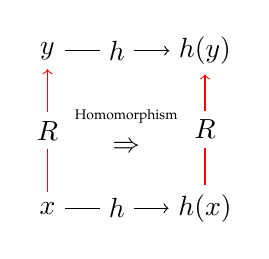
\begin{tikzpicture}[scale=2]
\node (x) at (0,0){$x$};
\node (y) at (0,1){$y$};
\node (fx) at (1,0){$h(x)$};
\node (fy) at (1,1){$h(y)$};
\node  at (.5,.5){\begin{tabular}{c}{\tiny Homomorphism} \\ $\Rightarrow$\end{tabular}};
\draw[->] (x)	--	(fx) 	node[midway, fill=white]{$h$};
\draw[->] (y)	--	(fy) 	node[midway, fill=white]{$h$};
\draw[->,red] (x)	--	(y)		node[black, midway, fill=white]{$R$};
\draw[->,red] (fx)	--	(fy)	node[black, midway, fill=white]{$R$};
\end{tikzpicture}\]
\end{frame}

%%%%%%%%%%%%%%%%%%%%%%%%%%%%%%%%%%%%%%%%%%%%%%%%%%%%%%%%%%%%%%%%%%%%%%%%%%%%%%%%%%%%%%%%%%%%%%%%%%%5

\begin{frame}
\frametitle{Zig-zag-morphisms}
\emph{Zig-zag-morphisms} $h$ from $\mathfrak M$ to $\mathfrak M'$ are homomorphisms $h:W\to W'$ satisfying the same atoms and making zags:
	\[ \begin{array}{rcl} 	%w\in v(p) &\Rightarrow &h(w) \in v'(p)\\
							\mathfrak M, w\models p &\Longleftarrow & \mathfrak M' , h(w) \models p \end{array}\]
\[ h(x)R'y' \Rightarrow (\exists y\seenby x) h(y) =y' \]
\[\hspace{3cm}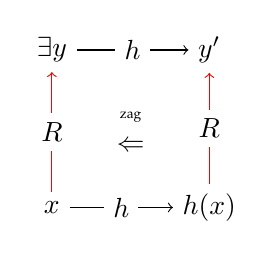
\begin{tikzpicture}[scale=2]
\node (x) at (0,0){$x$};
\node (y) at (0,1){$\exists y$};
\node (fx) at (1,0){$h(x)$};
\node (fy) at (1,1){$y'$};
\node  at (.5,.5){\begin{tabular}{c}{\tiny zag} \\ $\Leftarrow$\end{tabular}};
\draw[->] (x)	--	(fx) 	node[midway, fill=white]{$h$};
\draw[->] (y)	--	(fy) 	node[midway, fill=white]{$h$};
\draw[->,red] (x)	--	(y)		node[black, midway, fill=white]{$R$};
\draw[->,red] (fx)	--	(fy)	node[black, midway, fill=white]{$R$};
\end{tikzpicture}
\qquad
\uncover<2->{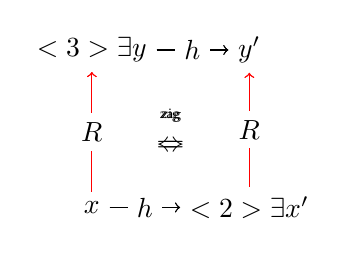
\begin{tikzpicture}[scale=2]
\node (x) at (0,0){$x$};
\node (y) at (0,1){$\uncover<3>{\exists}y$};
\node (fx) at (1,0){$\uncover<2>{\exists} x'$};
\node (fy) at (1,1){$y'$};
\uncover<2>{\node  at (.5,.5){\begin{tabular}{c}{\tiny zig} \\ $\Rightarrow$\end{tabular}};}
\uncover<2>{\draw[->, dashed] (x)	--	(fx) 	node[midway, fill=white]{$h$};}
\uncover<2>{\draw[->] (y)	--	(fy) 	node[midway, fill=white]{$h$};}
\uncover<2>{\draw[->,red] (x)	--	(y)		node[black, midway, fill=white]{$R$};}
\uncover<2>{\draw[->,red, dashed] (fx)	--	(fy)	node[black, midway, fill=white]{$R$};}
\uncover<3>{\node  at (.5,.5){\begin{tabular}{c}{\tiny zag} \\ $\Leftarrow$\end{tabular}};}
\uncover<3>{\draw[->] (x)	--	(fx) 	node[midway, fill=white]{$h$};}
\uncover<3>{\draw[->, dashed] (y)	--	(fy) 	node[midway, fill=white]{$h$};}
\uncover<3>{\draw[->,red, dashed] (x)	--	(y)		node[black, midway, fill=white]{$R$};}
\uncover<3>{\draw[->,red] (fx)	--	(fy)	node[black, midway, fill=white]{$R$};}
\end{tikzpicture}} \]
Zig-zags = The upward arrows ($R$) force each other out.


\end{frame}

%%%%%%%%%%%%%%%%%%%%%%%%%%%%%%%%%%%%%%%%%%%%%%%%%%%%%%%%%%%%%%%%%%%%%%%%%%%%%%%%%%%%%%%%%%%%%%%%%%%5

\begin{frame}
\frametitle{Invariance of truth}
\scriptsize
Truth is preserved under zig-zag-mapping.
\[ \mathfrak M , w \models \varphi \iff \mathfrak M' , h(w) \models \varphi \]

%\begin{multline*}
\textup{So $\varphi$
is true in a world of a model} %\\
\cemph{\textup{iff}} %\\
\textup{it is true in the zig-zag image of it.}
%\end{multline*}

\medskip
\hrule
\medskip

\dzsa{proof} By structural induction:
\begin{enumerate}\scriptsize
	\item atoms $p$:\qquad  $\mathfrak M , w \models p \iff \mathfrak M' , h(w) \models p$ -- but that's how we defined it!
	\item negations $\lnot\varphi$:
		\[ \begin{array}{ccccc}
		\mathfrak M , w \models \lnot \varphi
		&  \iff
		& \mathfrak M , h(w) \models \lnot \varphi
\\		\Updownarrow && \Updownarrow
\\[-1em]		\mathfrak M' , w \not \models \varphi
		&	\magyarazat{\iff}{ind.hip.}
		&	\mathfrak M , h(w) \not \models \varphi
		\end{array}\]
	\item conjunctions $\varphi \land\psi$: pretty much the same
	\item $\Diamond \varphi$:
		{\footnotesize
		\[ \begin{array}{ccccc}
		\mathfrak M , w \models \Diamond \varphi
		&  \iff
		&	\mathfrak M' , h(w) \models \Diamond \varphi
\\		\Updownarrow && \Updownarrow
\\[-1em]		(\exists v\seenby w)\; \mathfrak M , v \models \varphi
		&	\only<1>{\magyarazat{\Rightarrow}{zig+ind.hip.}}
						\only<2>{\magyarazat{\Leftarrow}{zag+ind.hip.}}
		&	(\only<1>{h(v)}\only<2>{\exists u}\seenby h(w)) \mathfrak M , h(\only<1>{v}\only<2>{u}) \models \varphi
		\end{array}\]}
\end{enumerate}
\end{frame}

%%%%%%%%%%%%%%%%%%%%%%%%%%%%%%%%%%%%%%%%%%%%%%%%%%%%%%%%%%%%%%%%%%%%%%%%%%%%%%%%%%%%%%%%%%%%%%%%%%%5

\begin{frame}
\frametitle{Invariance of validity}
Frame-validity is invariant under \underline{\emph{surjective}} zig-zag-mapping:
\[ \mathfrak F \models \varphi \iff h(\mathfrak F) \models \varphi \]

%\begin{multline*}
\textup{So $\varphi$
is valid on all zig-zag image } \cemph{iff} \textup{it is valid on the original.}
%\end{multline*}

\dzsa{proof}
{\footnotesize
	\[ \begin{array}{ccccc}
		\mathfrak F \not \models \varphi 	& 	\iff 	& h(\mathfrak F) \not \models \varphi
	\\[1em] 	\Updownarrow & & \Updownarrow
	\\ 	\exists V\;\underbrace{\mathfrak F, V}_{\mathfrak M}, w \not \models \varphi & 	\magyarazat{\iff}{inv.of.truth.} 	& \exists V' \; h(\mathfrak F),  V', h(w) \not \models \varphi
		\end{array}\]}

Here the $V$ and $V'$ are given by different reasons if we consider the different directions of the proof. One is given by the non-validity, and the other is determined by that; it is chosen to make a model zig-zag morphism from the frame zig-zag morphism $h$.
\end{frame}

%%%%%%%%%%%%%%%%%%%%%%%%%%%%%%%%%%%%%%%%%%%%%%%%%%%%%%%%%%%%%%%%%%%%%%%%%%%%%%%%%%%%%%%%%%%%%%%%%%%5

\begin{frame}
\frametitle{Invariance of validity}
Frame-validity is invariant under \emph{surjective} zig-zag-mapping:
\[ \mathfrak F \models \varphi \iff h(\mathfrak F) \models \varphi \]

%\begin{multline*}
\textup{So $\varphi$
is valid on all zig-zag image } \cemph{iff} \textup{it is valid on the original.}
%\end{multline*}

\dzsa{proof}
{\footnotesize
	\[ \begin{array}{ccccc}
		\mathfrak F \not \models \varphi 	& 	\iff 	& h(\mathfrak F) \not \models \varphi
	\\[1em] 	\Updownarrow & & \Updownarrow
	\\ 	\exists V\;\underbrace{\mathfrak F, V}_{\mathfrak M}, w \not \models \varphi & 	\magyarazat{\iff}{inv.of.truth.} 	& \exists V' \; h(\mathfrak F),  V', h(w) \not \models \varphi
		\end{array}\]}

Here the $V$ and $V'$ are given by different reasons if we consider the different directions of the proof. One is given by the non-validity, and the other is determined by that; it is chosen to make a model zig-zag morphism from the frame zig-zag morphism $h$.
\end{frame}

%%%%%%%%%%%%%%%%%%%%%%%%%%%%%%%%%%%%%%%%%%%%%%%%%%%%%%%%%%%%%%%%%%%%%%%%%%%%%%%%%%%%%%%%%%%%%%%%%%%5

\begin{frame}
\frametitle{Example}

\[ h: (\mathbb N, suc) \twoheadrightarrow (\{\bullet \}, \{(\bullet, \bullet)\})\]
\[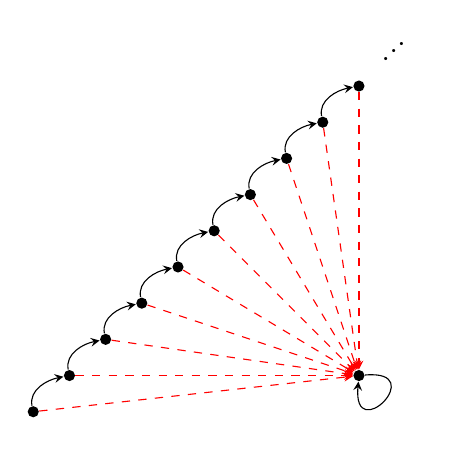
\begin{tikzpicture}[world/.style={inner sep=.5mm, fill=black, circle},>=stealth, rotate=-45, scale=1.3]

\node[world](bullet) at (0,0){};
\draw[->] (bullet) .. controls (50:.7cm) and (-50:.7cm) .. (bullet);

\node(11) at (-2,11*.5-3){\rotatebox{45}{\dots}};
\foreach \i in {1,2,...,10}{
\node[world](\i) at (-2,\i*.5-3){};
\draw[->, red, dashed] (\i) --(bullet);
}

\foreach \i in {1,2,...,9}{
\pgfmathtruncatemacro{\suci}{\i+1}
\draw[->](\i) edge[out=135, in=-135] (\suci);
}
\end{tikzpicture}\]

this proves that irreflexivity is not definable! If there is a formula defining that property, then that should be valid on $(\mathbb N, <)$, and its validity should be preserved under $h$ -- so that formula would be valid on a reflexive frame, and that is wrong.
\pause
\hazi{2}{1}{.7}{4}{0}{\begin{minipage}{3cm}Prove that antisymmetry and intransitivity is not definable.\end{minipage}}
\end{frame}

%%%%%%%%%%%%%%%%%%%%%%%%%%%%%%%%%%%%%%%%%%%%%%%%%%%%%%%%%%%%%%%%%%%%%%%%%%%%%%%%%%%%%%%%%%%%%%%%%%%5

\szakasz[Completeness]{Completeness}

\begin{frame}
\frametitle{Freedom}

$\mathfrak M $ is \emph{freer} than $\mathfrak M'$ iff $\mathfrak M$ has less truth then $\mathfrak M'$, i.e.,
\[\mathrm{Th} (\mathfrak M) \subseteq \mathrm{Th}(\mathfrak M') \quad \textup{where} \quad \mathrm{Th}(\mathfrak M )\defegy \{\varphi \, :\, \mathfrak M \models \varphi\}\]

Are there models $\mathfrak M$ that are \emph{absolutely free}, i.e.,
\[ \forall \mathfrak M' \qquad \mathrm{Th} (\mathfrak M) \subseteq \mathrm{Th}(\mathfrak M') \]

That would mean that such an absolutely free model is \emph{free from any contingencies} that are definable in the modal language. If something can be falsified in some model, then it will be false in the absolutely free one as well. Therefore, such a model would act like a \emph{universal countermodel}.

\end{frame}

%%%%%%%%%%%%%%%%%%%%%%%%%%%%%%%%%%%%%%%%%%%%%%%%%%%%%%%%%%%%%%%%%%%%%%%%%%%%%%%%%%%%%%%%%%%%%%%%%%%5

\begin{frame}
\frametitle{Characterization}

The minimal temporal logic is $\mathbf K \defegy \{ \varphi \, :\, \forall \mathfrak F \; \mathfrak F \models \varphi  \} $, i.e., the set of validities of frames in general. How can we create a logic from a set of formulas?

\bigskip

We will write $\models_{\mathbf K} \varphi $ instead of $\varphi \in \mathbf K$.

\bigskip

We will write $\psi_1, \dots , \psi_n \models_{\mathbf K} \varphi $ instead of $\models_{\mathbf K} (\psi_1\land \dots \land \psi_n) \lthen \varphi $.

\bigskip

We will write $\Gamma \models_{\mathbf K} \varphi $ instead of $\existsin {\psi_1, \dots , \psi_n}{\Gamma} \; \psi_1, \dots , \psi_n \models_{\mathbf K} \varphi $.

\bigskip

An absolutely free model $\mathfrak M$ then \emph{characterizes} $\mathbf{K}$:
\[ \mathfrak M \models \varphi \iff \models_{\mathbf K}  \varphi \]

\bigskip

So ``valid on every frame'' = ``true on $\mathfrak M$''.

\end{frame}

%%%%%%%%%%%%%%%%%%%%%%%%%%%%%%%%%%%%%%%%%%%%%%%%%%%%%%%%%%%%%%%%%%%%%%%%%%%%%%%%%%%%%%%%%%%%%%%%%%%5


\begin{frame}
\frametitle{Completeness}

It would be an interesting/important question whether $\mathbf K$, the logic of all frames, is finitely axiomatizable or not, i.e.,

\bigskip

is there a finite list of axioms and rules with which one could derive all the validities of $\mathbf K$? Or in other words,

\bigskip

is there a finite syntactical characterization of that logic too?

\end{frame}

%%%%%%%%%%%%%%%%%%%%%%%%%%%%%%%%%%%%%%%%%%%%%%%%%%%%%%%%%%%%%%%%%%%%%%%%%%%%%%%%%%%%%%%%%%%%%%%%%%%5

\begin{frame}
\frametitle{A concrete free model}
We will construct an absolutely free model $\mathfrak M_\mathbf K$ \cemph{ from $\mathbf{K}$}. In other words, we will construct a model whose
\begin{itemize}
\item every world will be a syntactical object: a special set of formulas.
\item alternative relation will be a syntactical relation: some special subset of that formula set is a subset of another one.
\item valuation will be given by the membership relation: for an atomic sentence,
\begin{multline*}
\textup{\cemph{to be \emph{true} in a set of formulas}} \\ \textup{\cemph{ is the same as }} \\ \textup{ \cemph{to be \emph{in} that set of formulas }}\end{multline*}
\end{itemize}
We will invent the alternative relation and the notion of worlds in a way to make this property true for any kind of formulas, not only for the atoms, so to prove a statement like this

\[ \varphi \in \Gamma \iff \mathfrak M_{\mathbf K}, \Gamma \models \varphi \]

This will be the so-called \emph{free} model of $\mathbf K$, the property above will be called \emph{Truth Lemma}.

\end{frame}

%%%%%%%%%%%%%%%%%%%%%%%%%%%%%%%%%%%%%%%%%%%%%%%%%%%%%%%%%%%%%%%%%%%%%%%%%%%%%%%%%%%%%%%%%%%%%%%%%%%5


\begin{frame}
\frametitle{A free model of $\mathbf K$}

\[\mathfrak M_{\mathbf K} \defegy \left( W_{\mathbf K}, R_{\mathbf K}, V_{\mathbf K}\right)   \]
where
\begin{itemize}
\item $W_{\mathbf K} \defegy \{\Gamma \, :\, \textup{$ \Gamma$  is a maximally $\mathbf K$-consistent set} \}$, i.e.,
\begin{itemize}\footnotesize
\item Every $\Gamma$ is $\mathbf K$-consistent: $\Gamma \not \models_{\mathbf K} \bot$
\item These $\Gamma$'s is so huge that if you try to put one more formula in it, you would make it $\mathbf K$-inconsistent:
\[ \forallp {\varphi\not \ni \Gamma} \quad \Gamma \cup \{\varphi \}\models_{\mathbf K}\bot\]
\end{itemize}
\item $\Gamma R_{\mathbf K}\Gamma'$ iff $\Gamma'$ contains $\varphi$ whenever $\Gamma$ contains $\FB \varphi$, formally:
 \[ \Gamma R_{\mathbf K}\Gamma' \defekv \FB^-(\Gamma )\subseteq \Gamma' \qquad \qquad \textup{ where }\FB^-(\Gamma)\defegy \{\varphi \, : \, \FB \varphi \in \Gamma\}\]
\item $\Gamma \in V_{\mathbf K}(p) \defekv p\in \Gamma$
\end{itemize}


\end{frame}

%%%%%%%%%%%%%%%%%%%%%%%%%%%%%%%%%%%%%%%%%%%%%%%%%%%%%%%%%%%%%%%%%%%%%%%%%%%%%%%%%%%%%%%%%%%%%%%%%%%5


\begin{frame}
\frametitle{free alternative relation}
The followings are equivalent:

\begin{itemize}
\item $\Gamma R_{\mathbf K}\Gamma'$
\item  $\Gamma'$ contains $\alpha$ whenever $\Gamma$ contains $\FB \alpha$, formally:
 \[ \FB^-(\Gamma )\subseteq \Gamma' \qquad \qquad \textup{ where }\FB^-(\Gamma)\defegy \{\alpha \, : \, \FB \alpha \in \Gamma\}\]
\item  $\Gamma$ contains $\FD\beta$ whenever $\Gamma'$ contains $\beta$, formally:
 \[ \Gamma \supseteq \FD^+(\Gamma') \qquad \qquad \textup{ where }\FD^+(\Gamma')\defegy \{\FD \beta \, : \, \beta \in \Gamma'\}\]
\item  $\Gamma$ contains $\gamma$ whenever $\Gamma'$ contains $\PB \gamma$, formally:
 \[ \Gamma \supseteq \PB^-(\Gamma') \qquad \qquad \textup{ where }\PB^-(\Gamma')\defegy \{\gamma \, : \, \PB \gamma \in \Gamma'\}\]
\item  $\Gamma'$ contains $\PD\delta$ whenever $\Gamma$ contains $\delta$, formally:
 \[  \PD^+(\Gamma)\subseteq \Gamma' \qquad \qquad \textup{ where }\PD^+(\Gamma)\defegy \{\PD \delta \, : \, \delta \in \Gamma\}\]
\end{itemize}


\end{frame}

%%%%%%%%%%%%%%%%%%%%%%%%%%%%%%%%%%%%%%%%%%%%%%%%%%%%%%%%%%%%%%%%%%%%%%%%%%%%%%%%%%%%%%%%%%%%%%%%%%%5

\begin{frame}
\frametitle{free alternative relation}
 \[ \PD^+(\Gamma)\subseteq \Gamma'  \Rightarrow \FB^-(\Gamma )\subseteq \Gamma'  \qquad\qquad\qquad \Gamma \supseteq \FD^+(\Gamma') \Rightarrow \Gamma \supseteq \PB^-(\Gamma') \]
\hrule
\medskip
\[\begin{array}{ll}
   \FB \varphi \in \Gamma& \textup{assumption}
\\ \PD\FB \varphi \in \Gamma' & \textup{by $\PD^+(\Gamma)\subseteq \Gamma' $}
\\ \varphi \in \Gamma' & \textup{because $\models_{\mathbf K} \PD\FB\varphi \lthen \varphi$}
\end{array}
\qquad
\begin{array}{ll}
%\\ \textsc{Proof}\\
\PB \varphi \in \Gamma'& \textup{assumption}
\\ \FD\PB \varphi \in \Gamma & \textup{by $\Gamma \supseteq \FD^+(\Gamma')$}
\\ \varphi \in \Gamma & \textup{because $\models_{\mathbf K} \FD\PB\varphi \lthen \varphi$}
\end{array}
\]

\pause
\hazi{2}{1}{.7}{5}{-4}{\begin{minipage}{3cm}Prove the remaining directions!\end{minipage}}
\hazi{2}{1}{.7}{0}{-4}{\begin{minipage}{3cm}Prove that \\ $\models_{\mathbf K} \PD\FB\varphi \lthen \varphi$ and \\ $\models_{\mathbf K} \FD\PB\varphi \lthen \varphi$\end{minipage}}
\end{frame}

%%%%%%%%%%%%%%%%%%%%%%%%%%%%%%%%%%%%%%%%%%%%%%%%%%%%%%%%%%%%%%%%%%%%%%%%%%%%%%%%%%%%%%%%%%%%%%%%%%%5


\begin{frame}
\frametitle{Truth Lemma}

\[\varphi \in \Gamma \iff \mathfrak M_{\mathbf K}, \Gamma \models \varphi \]
\hrule
\medskip

\[\begin{array}{rcll}
p \in \Gamma &\iff& \Gamma \in V_\mathbf K (p) & \textup{by def. of $V_\mathbf K$}
\\ &\iff&\mathfrak M_{\mathbf K}, \Gamma \models \varphi& \textup{by def. of $\models$}
\\[1em] \lnot \varphi \in \Gamma &\iff& \varphi \notin \Gamma  & \textup{$\Gamma$ is consistent}
\\ &\iff&\mathfrak M_{\mathbf K}, \Gamma \not\models \varphi& \textup{ind.hip.}
\\ &\iff&\mathfrak M_{\mathbf K}, \Gamma \models \lnot \varphi& \textup{by def. of $\models$}
\\[1em] \varphi \land \psi \in \Gamma &\iff& \varphi\in \Gamma \textup{ and } \psi \in \Gamma & \textup{$\Gamma$ is maximally cons.}
\\ &\iff&\mathfrak M_{\mathbf K}, \Gamma \models \varphi \textup{ and } \mathfrak M_{\mathbf K}, \Gamma \models \psi& \textup{ind.hip.}
\\ &\iff&\mathfrak M_{\mathbf K}, \Gamma \models \varphi\land \psi& \textup{by def. of $\models$}
\end{array}\]

\end{frame}

%%%%%%%%%%%%%%%%%%%%%%%%%%%%%%%%%%%%%%%%%%%%%%%%%%%%%%%%%%%%%%%%%%%%%%%%%%%%%%%%%%%%%%%%%%%%%%%%%%%5

\begin{frame}
\frametitle{Truth Lemma}

\[\varphi \in \Gamma \iff \mathfrak M_{\mathbf K}, \Gamma \models \varphi \]
\hrule
\medskip

\[\begin{array}{rcll}
 \FB \varphi \in \Gamma  &\iff& \varphi \in \FB^-(\Gamma) & \textup{def.of $\FB^-$}
\\
\magyi{\begin{tabular}{c}
we should prove \\the other direction!
\end{tabular}}&\cemph{\Longrightarrow}& \forallin {\Gamma'}{W_\mathbf K} \big[\Gamma' \supseteq \FB^-(\Gamma) \\ &&\hfill \textup{ implies } \varphi \in \Gamma' \big]&
\\ &\iff& \forallp {\Gamma' \seenby_{\mathbf K} \Gamma}\; \varphi \in \Gamma' &\textup{def.of $R_\mathbf K$}
\\ &\iff& \forallp {\Gamma' \seenby_{\mathbf K} \Gamma}\; \mathfrak M_{\mathbf K}, \Gamma' \models \varphi& \textup{ind.hip.}
\\ &\iff&\mathfrak M_{\mathbf K}, \Gamma \models \FB \varphi& \textup{by def. of $\models$}
\\[1em]
\PB \varphi \in \Gamma  &\iff& \varphi \in \PB^-(\Gamma) & \textup{def.of $\PB^-$}
\\
\magyi{\begin{tabular}{c}
we should prove \\the other direction!
\end{tabular}}&\cemph{\Longrightarrow}& \forallin {\Gamma'}{W_\mathbf K} \big[\Gamma' \supseteq \PB^-(\Gamma) \\ &&\hfill \textup{ implies } \varphi \in \Gamma' \big]&
\\ &\iff& \forallin {\Gamma'}{W_\mathbf K} \big[\FB^-(\Gamma') \subseteq \Gamma \\ &&\hfill \textup{ implies } \varphi \in \Gamma' \big]&\magyi{the equivalences}
\\ &\iff& \forallp {\Gamma' R_{\mathbf K} \Gamma}\; \varphi \in \Gamma' &\textup{def.of $R_\mathbf K$}
\\ &\iff& \forallp {\Gamma' R_{\mathbf K} \Gamma}\; \mathfrak M_{\mathbf K}, \Gamma' \models \varphi& \textup{ind.hip.}
\\ &\iff&\mathfrak M_{\mathbf K}, \Gamma \models \PB \varphi& \textup{by def. of $\models$}
\end{array}\]

\end{frame}

%%%%%%%%%%%%%%%%%%%%%%%%%%%%%%%%%%%%%%%%%%%%%%%%%%%%%%%%%%%%%%%%%%%%%%%%%%%%%%%%%%%%%%%%%%%%%%%%%%%5


\begin{frame}
\frametitle{Existence Lemma}

\[\FB \varphi \in \Gamma  \iff \varphi \in \FB^-(\Gamma) \mathrel{\cemph{\Longleftarrow}} \forallin {\Gamma'}{W_\mathbf K} \big[\Gamma' \supseteq \FB^-(\Gamma) \textup{ implies } \varphi \in \Gamma' \big]\]
%\hrule
Take the contraposition instead!
\[\FB \varphi \notin \Gamma  \iff \varphi \notin \FB^-(\Gamma) \mathrel{\cemph{\Longrightarrow}} \existsin {\Gamma'}{W_\mathbf K} \big[\Gamma' \supseteq \FB^-(\Gamma) \textup{ and } \varphi \notin \Gamma' \big]\]
Since we have maximally consistent sets,
\[\lnot \FB \varphi \in \Gamma  \iff  \lnot\varphi \in \FB^-(\Gamma) \mathrel{\cemph{\Longrightarrow}} \existsin {\Gamma'}{W_\mathbf K} \big[\Gamma' \supseteq \FB^-(\Gamma) \textup{ and } \lnot \varphi \in \Gamma' \big]\]
Let $\varphi :=\lnot \psi$ (``if it is true for any $\varphi$, it is true for any negation $\lnot \psi$''):
\[\lnot \FB \lnot \psi \in \Gamma  \iff  \lnot\lnot \psi \in \FB^-(\Gamma) \mathrel{\cemph{\Longrightarrow}} \existsin {\Gamma'}{W_\mathbf K} \big[\Gamma' \supseteq \FB^-(\Gamma) \textup{ and } \lnot \lnot \psi \in \Gamma' \big]\]
i.e., our meditational object will be
\[\FD \psi \in \Gamma  \iff  \psi \in \FB^-(\Gamma) \mathrel{\cemph{\Longrightarrow}} \existsin {\Gamma'}{W_\mathbf K} \big[\Gamma' \supseteq \FB^-(\Gamma) \textup{ and } \psi \in \Gamma' \big]\]
So we have to prove that the presence of a $\FD\psi$ in a m.c.s. enforce the existence of an other, \emph{related} m.c.s. set, in which $\varphi$ is contained.
\end{frame}

%%%%%%%%%%%%%%%%%%%%%%%%%%%%%%%%%%%%%%%%%%%%%%%%%%%%%%%%%%%%%%%%%%%%%%%%%%%%%%%%%%%%%%%%%%%%%%%%%%%5

\begin{frame}
\frametitle{Existence Lemma}

\[\FD \psi \in \Gamma  \iff  \psi \in \FB^-(\Gamma) \mathrel{\cemph{\Longrightarrow}} \existsin {\Gamma'}{W_\mathbf K} \big[\Gamma' \supseteq \FB^-(\Gamma) \textup{ and } \psi \in \Gamma' \big]\]

\hrule
\medskip

$\FB^- (\Gamma) \cup \{\varphi\}$ is $\mathbf K$-consistent. For if
\[ \begin{tomb}{rcll}
   \FB^- (\Gamma) \cup \{\varphi\}&\models_{\mathbf K}&\bot &\textup{indirect assumption}
\\ \FB^- (\Gamma)&\models_{\mathbf K}& \lnot \varphi &\textup{Deduction theorem}
\\ \exists \chi_1,  \cdots,\chi_{n}&\models_{\mathbf K}& \lnot \varphi &\textup{def.of $\FB^- (\Gamma)\models_{\mathbf K}$}
\\ &\models_{\mathbf K}& (\chi_1 \land \dots \land \chi_{n}) \lthen \lnot \varphi &\textup{def.of $(\chi_1 \land \dots \land \chi_{n})\models_{\mathbf K}$}
\\ &\models_{\mathbf K}& \FB (\chi_1 \land \dots \land \chi_{n}) \lthen \FB \lnot \varphi &\textup{See below!}
\\ &\models_{\mathbf K}& (\FB \chi_1 \land \dots \land \FB\chi_{n})\lthen \FB \lnot \varphi &\textup{See below!}
\\ \FB \chi_1, \cdots ,\FB\chi_{n} &\models_{\mathbf K}& \FB \lnot \varphi & \textup{def.of $(\FB \chi_1 \land \dots \land \FB \chi_{n})\models_{\mathbf K}$}
\\ \Gamma &\models_{\mathbf K}& \FB \lnot \varphi &\chi\in \FB^-(\Gamma) \Leftrightarrow \FB \chi\in \Gamma
\\ \Gamma &\models_{\mathbf K}& \lnot \FD\varphi &\textup{Duality}
\\ \Gamma \cup \{ \FD\varphi \}&\models_{\mathbf K}& \bot &\textup{Deduction theorem}
\\ \Gamma &\models_{\mathbf K}& \bot &\textup{we assumed that $\FD \varphi \in \Gamma$}
\end{tomb}\]

Remember that we relied on basically the following two logical rule:

\[ \models_{\mathbf K}(\FB \varphi \land \FB \psi) \lthen \FB (\varphi \land \psi ) \qquad \qquad \begin{tomb}[0]{l} \models_{\mathbf K} \varphi \lthen \psi \\ \hline \models_{\mathbf K} \FB \varphi \lthen \FB \psi \end{tomb}\]

%\pause
%\hazi{2}{1}{.7}{5}{-4}{\begin{minipage}{3cm}Prove that these are valid indeed!\end{minipage}}
\end{frame}

%%%%%%%%%%%%%%%%%%%%%%%%%%%%%%%%%%%%%%%%%%%%%%%%%%%%%%%%%%%%%%%%%%%%%%%%%%%%%%%%%%%%%%%%%%%%%%%%%%%5

\begin{frame}
\frametitle{Existence Lemma}

\[\PD \psi \in \Gamma  \iff  \psi \in \PB^-(\Gamma) \mathrel{\cemph{\Longrightarrow}} \existsin {\Gamma'}{W_\mathbf K} \big[\Gamma' \supseteq \PB^-(\Gamma) \textup{ and } \psi \in \Gamma' \big]\]

\hrule
\medskip

$\PB^- (\Gamma) \cup \{\varphi\}$ is $\mathbf K$-consistent. For if
\[ \begin{tomb}{rcll}
   \PB^- (\Gamma) \cup \{\varphi\}&\models_{\mathbf K}&\bot &\textup{indirect assumption}
\\ \PB^- (\Gamma)&\models_{\mathbf K}& \lnot \varphi &\textup{Deduction theorem}
\\ \exists \chi_1,  \cdots,\chi_{n}&\models_{\mathbf K}& \lnot \varphi &\textup{def.of $\PB^- (\Gamma)\models_{\mathbf K}$}
\\ &\models_{\mathbf K}& (\chi_1 \land \dots \land \chi_{n}) \lthen \lnot \varphi &\textup{def.of $(\chi_1 \land \dots \land \chi_{n})\models_{\mathbf K}$}
\\ &\models_{\mathbf K}& \PB (\chi_1 \land \dots \land \chi_{n}) \lthen \PB \lnot \varphi &\textup{See below!}
\\ &\models_{\mathbf K}& (\PB \chi_1 \land \dots \land \PB\chi_{n})\lthen \PB \lnot \varphi &\textup{See below!}
\\ \PB \chi_1, \cdots ,\PB\chi_{n} &\models_{\mathbf K}& \PB \lnot \varphi & \textup{def.of $(\PB \chi_1 \land \dots \land \PB \chi_{n})\models_{\mathbf K}$}
\\ \Gamma &\models_{\mathbf K}& \PB \lnot \varphi &\chi\in \PB^-(\Gamma) \Leftrightarrow \PB \chi\in \Gamma
\\ \Gamma &\models_{\mathbf K}& \lnot \PD\varphi &\textup{Duality}
\\ \Gamma \cup \{ \PD\varphi \}&\models_{\mathbf K}& \bot &\textup{Deduction theorem}
\\ \Gamma &\models_{\mathbf K}& \bot &\textup{we assumed that $\PD \varphi \in \Gamma$}
\end{tomb}\]

Remember that we relied on basically the following two logical rule:

\[ \models_{\mathbf K}(\PB \varphi \land \PB \psi) \lthen \PB (\varphi \land \psi ) \qquad \qquad \begin{tomb}[0]{l} \models_{\mathbf K} \varphi \lthen \psi \\ \hline \models_{\mathbf K} \PB \varphi \lthen \PB \psi \end{tomb}\]
\pause
\hazi{2}{1}{.7}{5}{-4}{\begin{minipage}{3cm}Prove that these are valid indeed!\end{minipage}}
\end{frame}

%%%%%%%%%%%%%%%%%%%%%%%%%%%%%%%%%%%%%%%%%%%%%%%%%%%%%%%%%%%%%%%%%%%%%%%%%%%%%%%%%%%%%%%%%%%%%%%%%%%5


\begin{frame}
\frametitle{Lindenbaum's Lemma}

Since $\FB^- (\Gamma) \cup \{\varphi\}$ is $\mathbf K$-consistent, it can be extended into a maximally consistent set $\Gamma'$. Just list all the formulas and start the following procedure: take the first formula: Is it consistent with $\Sigma_0 \defegy \FB^- (\Gamma) \cup \{\varphi\} $? If it is, then extend $\Sigma_0$ with that formula, if not, then don't. Repeat this into the infinity. Your m.c.s. will be $\FB^- (\Gamma) \cup \{\varphi\}$ the one will contain every formula with which you would extend.

\[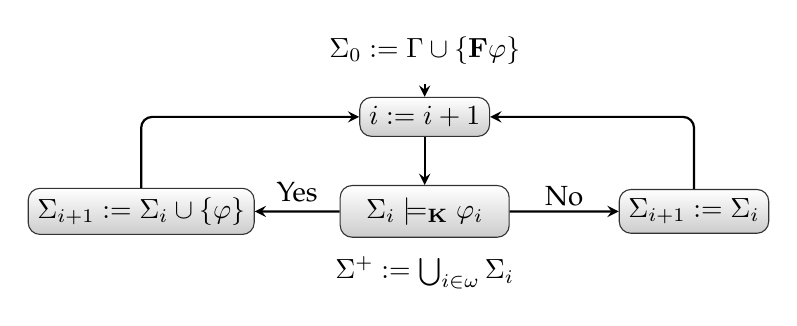
\begin{tikzpicture}[scale=1.2,>=stealth,
allapot/.style={ rectangle,rounded corners=1.5mm,draw=black!80,top color=white,bottom color=black!20,
}]

\pgfmathsetmacro{\magassag}{-1}

\node at (0,-3.8){$\Sigma_0 := \Gamma\cup\{\FD \varphi\}$ };


\begin{scope}[yshift=-4.5cm]
\node(0) at (0,.45){};
\node[allapot](i) at (0,0){$i:=i+1$};

\node[allapot](test) at (0,\magassag){\begin{tabular}{c}
  $\Sigma_i \models_{\mathbf{K}} \varphi_i$
\end{tabular}};

\node[allapot](yes-case) at (-3,\magassag){$\Sigma_{i+1} := \Sigma_i\cup \{\varphi\}$};

\node[allapot](no-case) at (2.85,\magassag){$\Sigma_{i+1} := \Sigma_i$};

\begin{scope}[->, thick, rounded corners=4pt]
\draw (0)--(i);
\draw (i)--(test);
\draw (test)--(no-case) node[pos=.5, above, inner sep=.5mm]{No};
\draw (test)--(yes-case)node[pos=.5, above, inner sep=1mm]{Yes};
\draw (yes-case)|-(i);
\draw (no-case)|-(i);
\end{scope}
\end{scope}

\node at (0,-6.15){$\Sigma^+ := \bigcup_{i\in \omega} \Sigma_i$ };

\end{tikzpicture}\]

Similarly for $\PB$.

\pause
\hazi{2}{1}{.7}{5}{-4}{\begin{minipage}{3cm}Prove that $\Sigma^+$ must be consistent!\end{minipage}}
\end{frame}

%%%%%%%%%%%%%%%%%%%%%%%%%%%%%%%%%%%%%%%%%%%%%%%%%%%%%%%%%%%%%%%%%%%%%%%%%%%%%%%%%%%%%%%%%%%%%%%%%%%5


\begin{frame}
\frametitle{Absolute freedom / Characterization / free model theorem}
%\frametitle{$\mathfrak M_{\mathbf K}$ characterizes $\mathbf K$}
Only (Exactly) the valid formulas are true in $\mathfrak M_{\mathbf K}$.
\[ \mathfrak M_{\mathbf K} \models \varphi \iff \models_\mathbf K  \varphi \]
\hrule

\medskip

We show that
\[ \mathfrak M_{\mathbf K} \not\models \varphi \iff \not\models_\mathbf K  \varphi .\]
Since the construction called ``free model'' is a real \emph{model} indeed, we have the $\Rightarrow$ direction.

If $\not\models_\mathbf K \varphi$, then $\{\lnot \varphi\}$ is $\mathbf K$-consistent. Therefore we can extend it to a maximally $\mathbf K$-consistent $\Gamma^{\lnot \varphi}$ set by Lindenbaum's lemma. But this set is a world in the free model $\mathfrak M_\mathbf K$. And since this world contains $\lnot \varphi$, it is \emph{true} in it by the Truth lemma:
\[ \lnot \varphi \in \Gamma ^{\lnot \varphi} \Longrightarrow \mathfrak M _{\mathbf K} , \Gamma^{\lnot \varphi} \models \lnot \varphi \]
And we are ready, since we found a world of $\mathfrak M_\mathbf K$ where $\lnot \varphi$ is true, i.e., $\varphi$ is not true neither in that world nor in the whole model.

\end{frame}

%%%%%%%%%%%%%%%%%%%%%%%%%%%%%%%%%%%%%%%%%%%%%%%%%%%%%%%%%%%%%%%%%%%%%%%%%%%%%%%%%%%%%%%%%%%%%%%%%%%5

\begin{frame}[t]
\frametitle{Completeness}
Consider the following tautology:

\begin{center}Every non-$\mathbf K$-valid formula is falsifiable on some model\end{center}

A completeness theorem has a similar form:

\begin{center}Every non-$\mathbf K$-\cemph{theorem} is falsifiable on some model\end{center}
where the word ``theorem'' refers to some syntactic derivation system.

Using the absolute freedom of $\mathfrak M_{\mathbf K}$, we can freely interchange the second part of that sentence even in that opaque environment:

\begin{center}Every non-$\mathbf K$-\cemph{theorem} is falsifiable on the free model $\mathfrak M_{\mathbf K}$\end{center}

So we would have a finite syntactic characterization/axiomatization of $\mathbf K$ if we can define a finite derivational system satisfying that sentence.
Remember that we used only the validity of the following temporal formulas and rules:

\[ \PD\FB\varphi \lthen \varphi\qquad \FD\PB\varphi \lthen \varphi \]
\[ (\FB\varphi \land \FB \psi )\lthen \FB(\varphi \land \psi ) \qquad (\PB\varphi \land \PB \psi )\lthen \PB(\varphi \land \psi ) \]
\[ \lrule{\varphi \lthen \psi }{\FB\varphi \lthen \FB\psi } \qquad \lrule{\varphi \lthen \psi }{\PB\varphi \lthen \PB\psi } \]

\end{frame}

%%%%%%%%%%%%%%%%%%%%%%%%%%%%%%%%%%%%%%%%%%%%%%%%%%%%%%%%%%%%%%%%%%%%%%%%%%%%%%%%%%%%%%%%%%%%%%%%%%%5


\begin{frame}[t]
\frametitle{Derivation for $\mathbf K$}
We define the derivation relation $\derives[\mathbf K]$ inductively: It is the smallest relation satisfying the followings:
\begin{itemize}
\item $\derives[K]\varphi \lthen .\psi \lthen \varphi$ for all $\varphi, \psi$,
\item $\derives[K]\varphi\lthen (\psi \lthen \chi) \lthen . (\varphi \lthen \psi) \lthen . \varphi \lthen \chi$ for all $\varphi, \psi, \chi$,
\item $\derives[K]\varphi \lthen \psi \lthen .\lnot \psi \lthen \lnot \varphi$ for all $\varphi, \psi$,
\item $\derives[K]\PD\FB\varphi \lthen \varphi $ for all $\varphi$,
\item $\derives[K]\FD\PB\varphi \lthen \varphi$ for all $\varphi$,
\item $\derives[K](\FB\varphi \land \FB \psi )\lthen \FB(\varphi \land \psi )$ for all $\varphi, \psi$,
\item $\derives[K](\PB\varphi \land \PB \psi )\lthen \PB(\varphi \land \psi )$ for all $\varphi, \psi$,
\item If $\derives[K]\varphi$ and  $\derives[K]\varphi \lthen \psi$ then $\derives[K]\psi$,
\item If $\derives[K]\varphi\lthen \psi$, then $\derives[K]\FB\varphi \lthen \FB\psi$,
\item If $\derives[K]\varphi\lthen \psi$, then $\derives[K]\PB\varphi \lthen \PB\psi$.
\end{itemize}
\[\begin{array}{rcl}
\psi_1, \dots , \psi_n\derives[\mathbf K]\varphi&\defekv & \derives[\mathbf K] (\psi_1 \land \dots \land \psi_n)\lthen \varphi
\\ \Gamma\derives[\mathbf K]\varphi&\defekv &(\exists \psi_1, \dots , \psi_n \in \Gamma) \psi_1, \dots , \psi_n\derives[\mathbf K]\varphi\end{array}\]
\end{frame}

%%%%%%%%%%%%%%%%%%%%%%%%%%%%%%%%%%%%%%%%%%%%%%%%%%%%%%%%%%%%%%%%%%%%%%%%%%%%%%%%%%%%%%%%%%%%%%%%%%%5

\begin{frame}[t]
\frametitle{Derivation for $\mathbf K$}
\dzsa{Theorem}
$\Gamma \derives[\mathbf K]\varphi$ iff there is a finite list of formulas (called \emph{proof}) such that for every formula of that list it is true that
\begin{itemize}
\item it is an axiom of $\mathbf K$
\item it is an element of $\Gamma$
\item it can be derived from previous list-members using a rule of $\mathbf K$.
\end{itemize}

\hazi{2}{1}{.7}{0}{-1}{\begin{minipage}{5cm}
You should try to prove it -- this theorem is one of those for which it is true that everybody see why is it true, but not everybody can prove it step by step.\end{minipage}}
\end{frame}

%%%%%%%%%%%%%%%%%%%%%%%%%%%%%%%%%%%%%%%%%%%%%%%%%%%%%%%%%%%%%%%%%%%%%%%%%%%%%%%%%%%%%%%%%%%%%%%%%%%5

\begin{frame}
\frametitle{Strong completeness}
\dzsa{Theorem}
\[\Gamma \derives[\mathbf K]\varphi \qquad \iff\qquad \Gamma \models_{\mathbf K}\varphi\]
\hrule
\medskip
To prove $\Leftarrow$, we show
\[\Gamma \not\derives[\mathbf K]\varphi \qquad \Longrightarrow \qquad \Gamma \not\models_{\mathbf K}\varphi\]
From the premise we have $\Gamma \cup \{\lnot \varphi\}\not\derives[\mathbf K]\bot$. Then by replacing the sign $\models_{\mathbf K}$ with $\derives[\mathbf K]$ in Lindenbaum's lemma we can conclude that there is a maximally consistent set $\Sigma^{\Gamma \cup \{\lnot \varphi\}}$ that contains $\Gamma \cup \{\lnot \varphi\}$.
Now, again, replace $\models_{\mathbf K}$ with $\derives[\mathbf K]$ everywhere in the definition of the free model: The resulting construction will be called \emph{canonical model}. Since we used exactly the axioms of $\mathbf K$ in these proofs, we have the corresponding version of the free model theorem (called canonical model theorem) and the truth lemma as well. Then $\mathfrak M_\mathbf{K}$ has a world -- that would be $\Sigma^{\Gamma \cup \{\varphi\}}$ -- which contains every element of ${\Gamma \cup \{\lnot \varphi\}}$, therefore, by the truth lemma,
\[(\forall \psi \in \Gamma) \quad \mathfrak M_{\mathbf K}, \Sigma^{\Gamma \cup \{\varphi\}}\models \psi \qquad \textup{ but } \qquad\mathfrak M_{\mathbf K}, \Sigma^{\Gamma \cup \{\varphi\}}\not\models \varphi\]
So since the free model is a model, we have the desired counter model for $\Gamma \models_{\mathbf K}\varphi$.

\hazi{2}{1}{.7}{0}{-4.5}{\begin{minipage}{2cm}
Prove $\Rightarrow$.\end{minipage}}

\end{frame}

%%%%%%%%%%%%%%%%%%%%%%%%%%%%%%%%%%%%%%%%%%%%%%%%%%%%%%%%%%%%%%%%%%%%%%%%%%%%%%%%%%%%%%%%%%%%%%%%%%%5


\cimdia{Canonical model}

\begin{frame}
\frametitle{The canonical model}
We will construct an absolutely free model $\mathfrak M_\mathbf K$ \cemph{ from $\vdash_\mathbf{K}$}. In other words, we will construct a model whose
\begin{itemize}
\item every world will be a syntactical object: a special set of formulas.
\item alternative relation will be a syntactical relation: some special subset of that formula set is a subset of another one.
\item valuation will be given by the membership relation: for an atomic sentence,
\begin{multline*}
\textup{\cemph{to be \emph{true} in a set of formulas}} \\ \textup{\cemph{ is the same as }} \\ \textup{ \cemph{to be \emph{in} that set of formulas }}\end{multline*}
\end{itemize}
We will invent the alternative relation and the notion of worlds in a way to make this property true for any kind of formulas, not only for the atoms, so to prove a statement like this

\[ \varphi \in \Gamma \iff \mathfrak M_{\mathbf K}, \Gamma \models \varphi \]

This will be the so-called \emph{canonical} model of $\mathbf K$, the property above will be called \emph{Truth Lemma}.

\end{frame}


%%%%%%%%%%%%%%%%%%%%%%%%%%%%%%%%%%%%%%%%%%%%%%%%%%%%%%%%%%%%%%%%%%%%%%%%%%%%%%%%%%%%%%%%%%%%%%%%%%%5


\begin{frame}
\frametitle{A canonical model of $\mathbf K$}

\[\mathfrak M_{\mathbf K} \defegy \left( W_{\mathbf K}, R_{\mathbf K}, V_{\mathbf K}\right)   \]
where
\begin{itemize}
\item $W_{\mathbf K} \defegy \{\Gamma \, :\, \textup{$ \Gamma$  is a maximally $\mathbf K$-consistent set} \}$, i.e.,
\begin{itemize}\footnotesize
\item Every $\Gamma$ is $\mathbf K$-consistent: $\Gamma \not \vdash_{\mathbf K} \bot$
\item These $\Gamma$'s is so huge that if you try to put one more formula in it, you would make it $\mathbf K$-inconsistent:
\[ \forallp {\varphi\not \ni \Gamma} \quad \Gamma \cup \{\varphi \}\vdash_{\mathbf K}\bot\]
\end{itemize}
\item $\Gamma R_{\mathbf K}\Gamma'$ iff $\Gamma'$ contains $\varphi$ whenever $\Gamma$ contains $\FB \varphi$, formally:
 \[ \Gamma R_{\mathbf K}\Gamma' \defekv \FB^-(\Gamma )\subseteq \Gamma' \qquad \qquad \textup{ where }\FB^-(\Gamma)\defegy \{\varphi \, : \, \FB \varphi \in \Gamma\}\]
\item $\Gamma \in V_{\mathbf K}(p) \defekv p\in \Gamma$
\end{itemize}


\end{frame}

%%%%%%%%%%%%%%%%%%%%%%%%%%%%%%%%%%%%%%%%%%%%%%%%%%%%%%%%%%%%%%%%%%%%%%%%%%%%%%%%%%%%%%%%%%%%%%%%%%%5


\begin{frame}
\frametitle{canonical alternative relation}
The followings are equivalent:

\begin{itemize}
\item $\Gamma R_{\mathbf K}\Gamma'$
\item  $\Gamma'$ contains $\alpha$ whenever $\Gamma$ contains $\FB \alpha$, formally:
 \[ \FB^-(\Gamma )\subseteq \Gamma' \qquad \qquad \textup{ where }\FB^-(\Gamma)\defegy \{\alpha \, : \, \FB \alpha \in \Gamma\}\]
\item  $\Gamma$ contains $\FD\beta$ whenever $\Gamma'$ contains $\beta$, formally:
 \[ \Gamma \supseteq \FD^+(\Gamma') \qquad \qquad \textup{ where }\FD^+(\Gamma')\defegy \{\FD \beta \, : \, \beta \in \Gamma'\}\]
\item  $\Gamma$ contains $\gamma$ whenever $\Gamma'$ contains $\PB \gamma$, formally:
 \[ \Gamma \supseteq \PB^-(\Gamma') \qquad \qquad \textup{ where }\PB^-(\Gamma')\defegy \{\gamma \, : \, \PB \gamma \in \Gamma'\}\]
\item  $\Gamma'$ contains $\PD\delta$ whenever $\Gamma$ contains $\delta$, formally:
 \[  \PD^+(\Gamma)\subseteq \Gamma' \qquad \qquad \textup{ where }\PD^+(\Gamma)\defegy \{\PD \delta \, : \, \delta \in \Gamma\}\]
\end{itemize}


\end{frame}

%%%%%%%%%%%%%%%%%%%%%%%%%%%%%%%%%%%%%%%%%%%%%%%%%%%%%%%%%%%%%%%%%%%%%%%%%%%%%%%%%%%%%%%%%%%%%%%%%%%5

\begin{frame}
\frametitle{canonical alternative relation}
 \[ \PD^+(\Gamma)\subseteq \Gamma'  \Rightarrow \FB^-(\Gamma )\subseteq \Gamma'  \qquad\qquad\qquad \Gamma \supseteq \FD^+(\Gamma') \Rightarrow \Gamma \supseteq \PB^-(\Gamma') \]
\hrule
\medskip
\[\begin{array}{ll}
   \FB \varphi \in \Gamma& \textup{assumption}
\\ \PD\FB \varphi \in \Gamma' & \textup{by $\PD^+(\Gamma)\subseteq \Gamma' $}
\\ \varphi \in \Gamma' & \textup{because $\vdash_{\mathbf K} \PD\FB\varphi \lthen \varphi$}
\end{array}
\qquad
\begin{array}{ll}
%\\ \textsc{Proof}\\
\PB \varphi \in \Gamma'& \textup{assumption}
\\ \FD\PB \varphi \in \Gamma & \textup{by $\Gamma \supseteq \FD^+(\Gamma')$}
\\ \varphi \in \Gamma & \textup{because $\vdash_{\mathbf K} \FD\PB\varphi \lthen \varphi$}
\end{array}
\]

\pause
\hazi{2}{1}{.7}{5}{-4}{\begin{minipage}{3cm}Prove the remaining directions!\end{minipage}}
\hazi{2}{1}{.7}{0}{-4}{\begin{minipage}{3cm}Prove that \\ $\vdash_{\mathbf K} \PD\FB\varphi \lthen \varphi$ and \\ $\vdash_{\mathbf K} \FD\PB\varphi \lthen \varphi$\end{minipage}}
\end{frame}

%%%%%%%%%%%%%%%%%%%%%%%%%%%%%%%%%%%%%%%%%%%%%%%%%%%%%%%%%%%%%%%%%%%%%%%%%%%%%%%%%%%%%%%%%%%%%%%%%%%5


\begin{frame}
\frametitle{Truth Lemma}

\[\varphi \in \Gamma \iff \mathfrak M_{\mathbf K}, \Gamma \models \varphi \]
\hrule
\medskip

\[\begin{array}{rcll}
p \in \Gamma &\iff& \Gamma \in V_\mathbf K (p) & \textup{by def. of $V_\mathbf K$}
\\ &\iff&\mathfrak M_{\mathbf K}, \Gamma \models \varphi& \textup{by def. of $\models$}
\\[1em] \lnot \varphi \in \Gamma &\iff& \varphi \notin \Gamma  & \textup{$\Gamma$ is consistent}
\\ &\iff&\mathfrak M_{\mathbf K}, \Gamma \not\models \varphi& \textup{ind.hip.}
\\ &\iff&\mathfrak M_{\mathbf K}, \Gamma \models \lnot \varphi& \textup{by def. of $\models$}
\\[1em] \varphi \land \psi \in \Gamma &\iff& \varphi\in \Gamma \textup{ and } \psi \in \Gamma & \textup{$\Gamma$ is maximally cons.}
\\ &\iff&\mathfrak M_{\mathbf K}, \Gamma \models \varphi \textup{ and } \mathfrak M_{\mathbf K}, \Gamma \models \psi& \textup{ind.hip.}
\\ &\iff&\mathfrak M_{\mathbf K}, \Gamma \models \varphi\land \psi& \textup{by def. of $\models$}
\end{array}\]

\end{frame}

%%%%%%%%%%%%%%%%%%%%%%%%%%%%%%%%%%%%%%%%%%%%%%%%%%%%%%%%%%%%%%%%%%%%%%%%%%%%%%%%%%%%%%%%%%%%%%%%%%%5


\begin{frame}
\frametitle{Truth Lemma}

\[\varphi \in \Gamma \iff \mathfrak M_{\mathbf K}, \Gamma \models \varphi \]
\hrule
\medskip

\[\begin{array}{rcll}
 \FB \varphi \in \Gamma  &\iff& \varphi \in \FB^-(\Gamma) & \textup{def.of $\FB^-$}
\\
\magyi{\begin{tabular}{c}
we should prove \\the other direction!
\end{tabular}}&\cemph{\Longrightarrow}& \forallin {\Gamma'}{W_\mathbf K} \big[\Gamma' \supseteq \FB^-(\Gamma) \\ &&\hfill \textup{ implies } \varphi \in \Gamma' \big]&
\\ &\iff& \forallp {\Gamma' \seenby_{\mathbf K} \Gamma}\; \varphi \in \Gamma' &\textup{def.of $R_\mathbf K$}
\\ &\iff& \forallp {\Gamma' \seenby_{\mathbf K} \Gamma}\; \mathfrak M_{\mathbf K}, \Gamma' \models \varphi& \textup{ind.hip.}
\\ &\iff&\mathfrak M_{\mathbf K}, \Gamma \models \FB \varphi& \textup{by def. of $\models$}
\\[1em]
\PB \varphi \in \Gamma  &\iff& \varphi \in \PB^-(\Gamma) & \textup{def.of $\PB^-$}
\\
\magyi{\begin{tabular}{c}
we should prove \\the other direction!
\end{tabular}}&\cemph{\Longrightarrow}& \forallin {\Gamma'}{W_\mathbf K} \big[\Gamma' \supseteq \PB^-(\Gamma) \\ &&\hfill \textup{ implies } \varphi \in \Gamma' \big]&
\\ &\iff& \forallin {\Gamma'}{W_\mathbf K} \big[\FB^-(\Gamma') \subseteq \Gamma \\ &&\hfill \textup{ implies } \varphi \in \Gamma' \big]&\magyi{the equivalences}
\\ &\iff& \forallp {\Gamma' R_{\mathbf K} \Gamma}\; \varphi \in \Gamma' &\textup{def.of $R_\mathbf K$}
\\ &\iff& \forallp {\Gamma' R_{\mathbf K} \Gamma}\; \mathfrak M_{\mathbf K}, \Gamma' \models \varphi& \textup{ind.hip.}
\\ &\iff&\mathfrak M_{\mathbf K}, \Gamma \models \PB \varphi& \textup{by def. of $\models$}
\end{array}\]

\end{frame}

%%%%%%%%%%%%%%%%%%%%%%%%%%%%%%%%%%%%%%%%%%%%%%%%%%%%%%%%%%%%%%%%%%%%%%%%%%%%%%%%%%%%%%%%%%%%%%%%%%%5

\begin{frame}
\frametitle{Existence Lemma}

\[\FB \varphi \in \Gamma  \iff \varphi \in \FB^-(\Gamma) \mathrel{\cemph{\Longleftarrow}} \forallin {\Gamma'}{W_\mathbf K} \big[\Gamma' \supseteq \FB^-(\Gamma) \textup{ implies } \varphi \in \Gamma' \big]\]
%\hrule
Take the contraposition instead!
\[\FB \varphi \notin \Gamma  \iff \varphi \notin \FB^-(\Gamma) \mathrel{\cemph{\Longrightarrow}} \existsin {\Gamma'}{W_\mathbf K} \big[\Gamma' \supseteq \FB^-(\Gamma) \textup{ and } \varphi \notin \Gamma' \big]\]
Since we have maximally consistent sets,
\[\lnot \FB \varphi \in \Gamma  \iff  \lnot\varphi \in \FB^-(\Gamma) \mathrel{\cemph{\Longrightarrow}} \existsin {\Gamma'}{W_\mathbf K} \big[\Gamma' \supseteq \FB^-(\Gamma) \textup{ and } \lnot \varphi \in \Gamma' \big]\]
Let $\varphi :=\lnot \psi$ (``if it is true for any $\varphi$, it is true for any negation $\lnot \psi$''):
\[\lnot \FB \lnot \psi \in \Gamma  \iff  \lnot\lnot \psi \in \FB^-(\Gamma) \mathrel{\cemph{\Longrightarrow}} \existsin {\Gamma'}{W_\mathbf K} \big[\Gamma' \supseteq \FB^-(\Gamma) \textup{ and } \lnot \lnot \psi \in \Gamma' \big]\]
i.e., our meditational object will be
\[\FD \psi \in \Gamma  \iff  \psi \in \FB^-(\Gamma) \mathrel{\cemph{\Longrightarrow}} \existsin {\Gamma'}{W_\mathbf K} \big[\Gamma' \supseteq \FB^-(\Gamma) \textup{ and } \psi \in \Gamma' \big]\]
So we have to prove that the presence of a $\FD\psi$ in a m.c.s. enforce the existence of an other, \emph{related} m.c.s. set, in which $\varphi$ is contained.
\end{frame}

%%%%%%%%%%%%%%%%%%%%%%%%%%%%%%%%%%%%%%%%%%%%%%%%%%%%%%%%%%%%%%%%%%%%%%%%%%%%%%%%%%%%%%%%%%%%%%%%%%%5

\begin{frame}
\frametitle{Existence Lemma}

\[\FD \psi \in \Gamma  \iff  \psi \in \FB^-(\Gamma) \mathrel{\cemph{\Longrightarrow}} \existsin {\Gamma'}{W_\mathbf K} \big[\Gamma' \supseteq \FB^-(\Gamma) \textup{ and } \psi \in \Gamma' \big]\]

\hrule
\medskip

$\FB^- (\Gamma) \cup \{\varphi\}$ is $\mathbf K$-consistent. For if
\[ \begin{tomb}{rcll}
   \FB^- (\Gamma) \cup \{\varphi\}&\vdash_{\mathbf K}&\bot &\textup{indirect assumption}
\\ \FB^- (\Gamma)&\vdash_{\mathbf K}& \lnot \varphi &\textup{Deduction theorem}
\\ \exists \chi_1,  \cdots,\chi_{n}&\vdash_{\mathbf K}& \lnot \varphi &\textup{def.of $\FB^- (\Gamma)\vdash_{\mathbf K}$}
\\ &\vdash_{\mathbf K}& (\chi_1 \land \dots \land \chi_{n}) \lthen \lnot \varphi &\textup{def.of $(\chi_1 \land \dots \land \chi_{n})\vdash_{\mathbf K}$}
\\ &\vdash_{\mathbf K}& \FB (\chi_1 \land \dots \land \chi_{n}) \lthen \FB \lnot \varphi &\textup{See below!}
\\ &\vdash_{\mathbf K}& (\FB \chi_1 \land \dots \land \FB\chi_{n})\lthen \FB \lnot \varphi &\textup{See below!}
\\ \FB \chi_1, \cdots ,\FB\chi_{n} &\vdash_{\mathbf K}& \FB \lnot \varphi & \textup{def.of $(\FB \chi_1 \land \dots \land \FB \chi_{n})\vdash_{\mathbf K}$}
\\ \Gamma &\vdash_{\mathbf K}& \FB \lnot \varphi &\chi\in \FB^-(\Gamma) \Leftrightarrow \FB \chi\in \Gamma
\\ \Gamma &\vdash_{\mathbf K}& \lnot \FD\varphi &\textup{Duality}
\\ \Gamma \cup \{ \FD\varphi \}&\vdash_{\mathbf K}& \bot &\textup{Deduction theorem}
\\ \Gamma &\vdash_{\mathbf K}& \bot &\textup{we assumed that $\FD \varphi \in \Gamma$}
\end{tomb}\]

Remember that we relied on basically the following two logical rule:

\[ \vdash_{\mathbf K}(\FB \varphi \land \FB \psi) \lthen \FB (\varphi \land \psi ) \qquad \qquad \begin{tomb}[0]{l} \vdash_{\mathbf K} \varphi \lthen \psi \\ \hline \vdash_{\mathbf K} \FB \varphi \lthen \FB \psi \end{tomb}\]

%\pause
%\hazi{2}{1}{.7}{5}{-4}{\begin{minipage}{3cm}Prove that these are valid indeed!\end{minipage}}
\end{frame}

%%%%%%%%%%%%%%%%%%%%%%%%%%%%%%%%%%%%%%%%%%%%%%%%%%%%%%%%%%%%%%%%%%%%%%%%%%%%%%%%%%%%%%%%%%%%%%%%%%%5

\begin{frame}
\frametitle{Existence Lemma}

\[\PD \psi \in \Gamma  \iff  \psi \in \PB^-(\Gamma) \mathrel{\cemph{\Longrightarrow}} \existsin {\Gamma'}{W_\mathbf K} \big[\Gamma' \supseteq \PB^-(\Gamma) \textup{ and } \psi \in \Gamma' \big]\]

\hrule
\medskip

$\PB^- (\Gamma) \cup \{\varphi\}$ is $\mathbf K$-consistent. For if
\[ \begin{tomb}{rcll}
   \PB^- (\Gamma) \cup \{\varphi\}&\vdash_{\mathbf K}&\bot &\textup{indirect assumption}
\\ \PB^- (\Gamma)&\vdash_{\mathbf K}& \lnot \varphi &\textup{Deduction theorem}
\\ \exists \chi_1,  \cdots,\chi_{n}&\vdash_{\mathbf K}& \lnot \varphi &\textup{def.of $\PB^- (\Gamma)\vdash_{\mathbf K}$}
\\ &\vdash_{\mathbf K}& (\chi_1 \land \dots \land \chi_{n}) \lthen \lnot \varphi &\textup{def.of $(\chi_1 \land \dots \land \chi_{n})\vdash_{\mathbf K}$}
\\ &\vdash_{\mathbf K}& \PB (\chi_1 \land \dots \land \chi_{n}) \lthen \PB \lnot \varphi &\textup{See below!}
\\ &\vdash_{\mathbf K}& (\PB \chi_1 \land \dots \land \PB\chi_{n})\lthen \PB \lnot \varphi &\textup{See below!}
\\ \PB \chi_1, \cdots ,\PB\chi_{n} &\vdash_{\mathbf K}& \PB \lnot \varphi & \textup{def.of $(\PB \chi_1 \land \dots \land \PB \chi_{n})\vdash_{\mathbf K}$}
\\ \Gamma &\vdash_{\mathbf K}& \PB \lnot \varphi &\chi\in \PB^-(\Gamma) \Leftrightarrow \PB \chi\in \Gamma
\\ \Gamma &\vdash_{\mathbf K}& \lnot \PD\varphi &\textup{Duality}
\\ \Gamma \cup \{ \PD\varphi \}&\vdash_{\mathbf K}& \bot &\textup{Deduction theorem}
\\ \Gamma &\vdash_{\mathbf K}& \bot &\textup{we assumed that $\PD \varphi \in \Gamma$}
\end{tomb}\]

Remember that we relied on basically the following two logical rule:

\[ \vdash_{\mathbf K}(\PB \varphi \land \PB \psi) \lthen \PB (\varphi \land \psi ) \qquad \qquad \begin{tomb}[0]{l} \vdash_{\mathbf K} \varphi \lthen \psi \\ \hline \vdash_{\mathbf K} \PB \varphi \lthen \PB \psi \end{tomb}\]
\pause
\hazi{2}{1}{.7}{5}{-4}{\begin{minipage}{3cm}Prove that these are valid indeed!\end{minipage}}
\end{frame}

%%%%%%%%%%%%%%%%%%%%%%%%%%%%%%%%%%%%%%%%%%%%%%%%%%%%%%%%%%%%%%%%%%%%%%%%%%%%%%%%%%%%%%%%%%%%%%%%%%%5


\begin{frame}
\frametitle{Lindenbaum's Lemma}

Since $\FB^- (\Gamma) \cup \{\varphi\}$ is $\mathbf K$-consistent, it can be extended into a maximally consistent set $\Gamma'$. Just list all the formulas and start the following procedure: take the first formula: Is it consistent with $\Sigma_0 \defegy \FB^- (\Gamma) \cup \{\varphi\} $? If it is, then extend $\Sigma_0$ with that formula, if not, then don't. Repeat this into the infinity. Your m.c.s. will be $\FB^- (\Gamma) \cup \{\varphi\}$ the one will contain every formula with which you would extend.

\[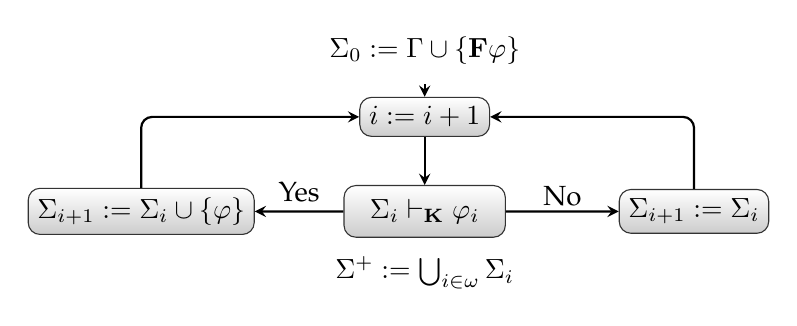
\begin{tikzpicture}[scale=1.2,>=stealth,
allapot/.style={ rectangle,rounded corners=1.5mm,draw=black!80,top color=white,bottom color=black!20,
}]

\pgfmathsetmacro{\magassag}{-1}

\node at (0,-3.8){$\Sigma_0 := \Gamma\cup\{\FD \varphi\}$ };


\begin{scope}[yshift=-4.5cm]
\node(0) at (0,.45){};
\node[allapot](i) at (0,0){$i:=i+1$};

\node[allapot](test) at (0,\magassag){\begin{tabular}{c}
  $\Sigma_i \vdash_{\mathbf{K}} \varphi_i$
\end{tabular}};

\node[allapot](yes-case) at (-3,\magassag){$\Sigma_{i+1} := \Sigma_i\cup \{\varphi\}$};

\node[allapot](no-case) at (2.85,\magassag){$\Sigma_{i+1} := \Sigma_i$};

\begin{scope}[->, thick, rounded corners=4pt]
\draw (0)--(i);
\draw (i)--(test);
\draw (test)--(no-case) node[pos=.5, above, inner sep=.5mm]{No};
\draw (test)--(yes-case)node[pos=.5, above, inner sep=1mm]{Yes};
\draw (yes-case)|-(i);
\draw (no-case)|-(i);
\end{scope}
\end{scope}

\node at (0,-6.15){$\Sigma^+ := \bigcup_{i\in \omega} \Sigma_i$ };

\end{tikzpicture}\]

Similarly for $\PB$.

\pause
\hazi{2}{1}{.7}{5}{-4}{\begin{minipage}{3cm}Prove that $\Sigma^+$ must be consistent!\end{minipage}}
\end{frame}

%%%%%%%%%%%%%%%%%%%%%%%%%%%%%%%%%%%%%%%%%%%%%%%%%%%%%%%%%%%%%%%%%%%%%%%%%%%%%%%%%%%%%%%%%%%%%%%%%%%5

\begin{frame}
\frametitle{Absolute freedom / Characterization / canonical model theorem}
%\frametitle{$\mathfrak M_{\mathbf K}$ characterizes $\mathbf K$}
Only (Exactly) the valid formulas are true in $\mathfrak M_{\mathbf K}$.
\[ \mathfrak M_{\mathbf K} \models \varphi \iff \vdash_\mathbf K  \varphi \]
\hrule

\medskip

We show that
\[ \mathfrak M_{\mathbf K} \not\models \varphi \iff \not\vdash_\mathbf K  \varphi .\]
Since the construction called ``canonical model'' is a real \emph{model} indeed, we have the $\Rightarrow$ direction.

If $\not\vdash_\mathbf K \varphi$, then $\{\lnot \varphi\}$ is $\mathbf K$-consistent. Therefore we can extend it to a maximally $\mathbf K$-consistent $\Gamma^{\lnot \varphi}$ set by Lindenbaum's lemma. But this set is a world in the canonical model $\mathfrak M_\mathbf K$. And since this world contains $\lnot \varphi$, it is \emph{true} in it by the Truth lemma:
\[ \lnot \varphi \in \Gamma ^{\lnot \varphi} \Longrightarrow \mathfrak M _{\mathbf K} , \Gamma^{\lnot \varphi} \models \lnot \varphi \]
And we are ready, since we found a world of $\mathfrak M_\mathbf K$ where $\lnot \varphi$ is true, i.e., $\varphi$ is not true neither in that world nor in the whole model.

\end{frame}

%%%%%%%%%%%%%%%%%%%%%%%%%%%%%%%%%%%%%%%%%%%%%%%%%%%%%%%%%%%%%%%%%%%%%%%%%%%%%%%%%%%%%%%%%%%%%%%%%%%5

\szakasz[Logics]{Logics}

\begin{frame}
\frametitle{Logic\cemph s}
\dzsa{Definition}
A \emph{normal temporal propositional logic} is a set of formulas that contains every $\mathbf K$-valid formula and is closed under the rules of $\mathbf K$.

\bigskip

\dzsa{Theorem}
$\mathbf K$ is the smallest normal temporal propositional logic.

\bigskip

\dzsa{Definition}
We denote the smallest normal temporal propositional logic that contains (the syntactically defined) $\mathbf K$ and $\varphi$ with $\mathbf K + (\varphi)$

\bigskip

\dzsa{Definition} A formula $\varphi$ is \emph{canonical} for a property $P$, iff besides that $\varphi$ is valid on $P$-frames, `by taking it as an axiom the canonical model of that new logic becomes $P$':
\[ \forallp {L\supseteq \mathbf K + (\varphi)} \textup{ $\mathfrak M _{L}$ has the property $P$} \]

\end{frame}

%%%%%%%%%%%%%%%%%%%%%%%%%%%%%%%%%%%%%%%%%%%%%%%%%%%%%%%%%%%%%%%%%%%%%%%%%%%%%%%%%%%%%%%%%%%%%%%%%%%5


\begin{frame}[t]
\frametitle{Axiomatizing Transitivity}
\footnotesize
\dzsa{Theorem} $\FB \varphi \lthen \FB \FB \varphi \quad \textup{ is canonical for }\quad w Rw'Rw'' \Rightarrow w R w''$

\bigskip

\dzsa{Proof} defining
Let $\mathrm{L}$ be a n.t.p. logic that contains the scheme \bemph{(4)} and let $\Gamma$, $\Gamma'$, $\Gamma''$  be arbitrary canonical worlds s.t. $\Gamma R_{\mathrm{L}} \Gamma' R_{\mathrm L} \Gamma''$. We have to prove that $\FB^-(\Gamma)\subseteq \Gamma''$. Take a $\FB\varphi \in \Gamma$. Then by \bemph{(4)}, $\FB\FB \varphi \in \Gamma$, therefore $\FB \varphi \in {\FB}^-(\Gamma)\subseteq \Gamma'$ and $\varphi \in {\FB}^-(\Gamma')\subseteq \Gamma''$.

\bigskip

\dzsa{Corollary} $\mathbf K + (4)$ axiomatizes the logic of transitive frames.


\begin{center}{\scriptsize (Because $\mathfrak M_{\mathbf K + (4)}$ will count as a counter-model.)}\end{center}
\end{frame}

%%%%%%%%%%%%%%%%%%%%%%%%%%%%%%%%%%%%%%%%%%%%%%%%%%%%%%%%%%%%%%%%%%%%%%%%%%%%%%%%%%%%%%%%%%%%%%%%%%%5

\begin{frame}[t]
\frametitle{Axiomatizing non-branching}
\footnotesize
\dzsa{Theorem}$ \PB (\PBDot \varphi \lthen \psi) \lor \PB (\PBDot \psi \lthen \varphi)$  is canonical for $( w Rw_1\textup{ and }w R w_2) \Rightarrow  (w_1 R w_2 \textup{ or } w_1 =  w_2 \textup{ or } w_1 \seenby w_2),$

\bigskip

\dzsa{Proof} Let $L$ be a n.t.p. logic containing the formula \bemph{(H.3)}.
Let $\Gamma$ be arbitrary but fixed, and let $\Gamma_1$ and $\Gamma_2$ be arbitrary $R_{\mathrm{L}}$-neighbours of $\Gamma$.

$\quad$ If $\Gamma_1=\Gamma_2$, then we are ready.
If $\Gamma_1\neq\Gamma_2$, then suppose indirectly that they are not related by $R_{\mathrm{L}}$ at all. That would mean that there is a formula $\PB \varphi\in \Gamma_1$ for which $\varphi \notin \Gamma_2$, and similarly, that there is a formula $\PB \psi\in \Gamma_2$ for which $\psi \notin \Gamma_1$. So $\PB \varphi, \lnot \psi \in \Gamma_1$ and $\PB \psi, \lnot \varphi \in \Gamma_2$.

$\quad$ In this case we would have that $\lnot(\PBDot \psi \lthen \varphi)\in \Gamma_1$ and $\lnot(\PBDot\varphi \lthen \psi)\in \Gamma_2 $, therefore, since both of $\Gamma_1$ and $\Gamma_2$ are $R_{\mathrm{L}}$-related to $\Gamma$ we have that $\PD\lnot(\PBDot \psi \lthen \varphi)\in \Gamma$ and $\PD  \lnot(\PBDot \varphi \lthen \psi)\in \Gamma$, i.e., even $\PD \lnot(\PBDot \psi \lthen \varphi)\land \PD \lnot(\PBDot \varphi \lthen \psi)\in \Gamma$, hence
$\lnot \PB (\PBDot \psi \lthen \varphi)\land \lnot \PB (\PBDot \varphi \lthen \psi)\in \Gamma$ which makes $\Gamma$ inconsistent.

\dzsa{Corollary}$\mathbf K + (H.3)$ axiomatizes the logic of those frames where there are no branching in the past.
\end{frame}

%%%%%%%%%%%%%%%%%%%%%%%%%%%%%%%%%%%%%%%%%%%%%%%%%%%%%%%%%%%%%%%%%%%%%%%%%%%%%%%%%%%%%%%%%%%%%%%%%%%5

\szakasz[Summary]{Short Summary}
\begin{frame}[t]
\frametitle{$\mathbf K$}
\framesubtitle{Logic of frames}
\footnotesize
\begin{minipage}[t]{6cm}
\begin{itemize}
\item[(PC1)] $\varphi \lthen .\psi \lthen \varphi$
\item[(PC2)] $\varphi\lthen (\psi \lthen \chi) \lthen . (\varphi \lthen \psi) \lthen . \varphi \lthen \chi$
\item[(PC3)] $\varphi \lthen \psi \lthen .\lnot \psi \lthen \lnot \varphi$
\item[(CP)] $\PD\FB\varphi \lthen \varphi $
\item[(CF)] $\FD\PB\varphi \lthen \varphi$
\item[(AP)] $(\FB\varphi \land \FB \psi )\lthen \FB(\varphi \land \psi )$
\item[(AF)] $(\PB\varphi \land \PB \psi )\lthen \PB(\varphi \land \psi )$
\item[(MP)] $\lrule {\varphi \\ \varphi \lthen \psi}{\psi}$
\item[(PLem)] $\lrule{\varphi\lthen \psi}{\PB\varphi \lthen \PB\psi}$
\item[(FLem)] $\lrule{\varphi\lthen \psi}{\FB\varphi \lthen \FB\psi}$
\end{itemize}
\end{minipage}
\felirat{5}{1}{.6}{3.5}{0}{ \begin{minipage}{7cm}
A more traditional axiomatization: replace the (AF)-(AP)-(PLem)-(FLem) schemes with %\\ this: \qquad

\medskip

\begin{itemize}
\item[(KP)]$ \PB(\varphi \lthen \psi )\lthen (\PB\varphi \lthen \PB \psi )$
\item[(KF)]$ \FB(\varphi \lthen \psi )\lthen (\FB\varphi \lthen \FB \psi )$
\item[(RNP)]$ \lrule{\varphi}{\PB \varphi}$
\item[(RNF)]$ \lrule{\varphi}{\FB \varphi}$
\end{itemize}

And it is also usual to postulate the duals (contrapositions) of (CP) and (CF)

\end{minipage}}

\end{frame}

%%%%%%%%%%%%%%%%%%%%%%%%%%%%%%%%%%%%%%%%%%%%%%%%%%%%%%%%%%%%%%%%%%%%%%%%%%%%%%%%%%%%%%%%%%%%%%%%%%%5

\begin{frame}[t]
\frametitle{$\mathbf K+ (4)$}
\framesubtitle{Logic of transitive frames}
\footnotesize
\begin{minipage}[t]{5.78cm}
\begin{itemize}
\item[(PC1)] $\varphi \lthen .\psi \lthen \varphi$
\item[(PC2)] $\varphi\lthen (\psi \lthen \chi) \lthen\!\!. (\varphi \lthen \psi) \lthen\!\! . \varphi \lthen \chi$
\item[(PC3)] $\varphi \lthen \psi \lthen .\lnot \psi \lthen \lnot \varphi$
\item[(CP)] $\PD\FB\varphi \lthen \varphi $
\item[(CF)] $\FD\PB\varphi \lthen \varphi$
\item[(AP)] $(\FB\varphi \land \FB \psi )\lthen \FB(\varphi \land \psi )$
\item[(AF)] $(\PB\varphi \land \PB \psi )\lthen \PB(\varphi \land \psi )$
\item[(MP)] $\lrule {\varphi \\ \varphi \lthen \psi}{\psi}$
\item[(PLem)] $\lrule{\varphi\lthen \psi}{\PB\varphi \lthen \PB\psi}$
\item[(FLem)] $\lrule{\varphi\lthen \psi}{\FB\varphi \lthen \FB\psi}$
\end{itemize}
\end{minipage}
\begin{minipage}[t]{4cm}
\begin{itemize}
\item[(4)] $\FB\varphi\lthen \FB\FB\varphi$
\end{itemize}
\end{minipage}
\end{frame}

%%%%%%%%%%%%%%%%%%%%%%%%%%%%%%%%%%%%%%%%%%%%%%%%%%%%%%%%%%%%%%%%%%%%%%%%%%%%%%%%%%%%%%%%%%%%%%%%%%%5

\begin{frame}[t]
\frametitle{$\mathbf K+ (\mathrm H.3)$}
\framesubtitle{Logic of backward-nonbranching frames}
\footnotesize
\begin{minipage}[t]{5.78cm}
\begin{itemize}
\item[(PC1)] $\varphi \lthen .\psi \lthen \varphi$
\item[(PC2)] $\varphi\lthen (\psi \lthen \chi) \lthen\!\!. (\varphi \lthen \psi) \lthen\!\! . \varphi \lthen \chi$
\item[(PC3)] $\varphi \lthen \psi \lthen .\lnot \psi \lthen \lnot \varphi$
\item[(CP)] $\PD\FB\varphi \lthen \varphi $
\item[(CF)] $\FD\PB\varphi \lthen \varphi$
\item[(AP)] $(\FB\varphi \land \FB \psi )\lthen \FB(\varphi \land \psi )$
\item[(AF)] $(\PB\varphi \land \PB \psi )\lthen \PB(\varphi \land \psi )$
\item[(MP)] $\lrule {\varphi \\ \varphi \lthen \psi}{\psi}$
\item[(PLem)] $\lrule{\varphi\lthen \psi}{\PB\varphi \lthen \PB\psi}$
\item[(FLem)] $\lrule{\varphi\lthen \psi}{\FB\varphi \lthen \FB\psi}$
\end{itemize}
\end{minipage}\quad
\begin{minipage}[t]{4.5cm}
\begin{itemize}
\item[(H.3)] $\PB(\PBDot \varphi\lthen \psi ) \lor \PB(\PBDot \psi\lthen \varphi )$
\end{itemize}
\end{minipage}
\end{frame}

%%%%%%%%%%%%%%%%%%%%%%%%%%%%%%%%%%%%%%%%%%%%%%%%%%%%%%%%%%%%%%%%%%%%%%%%%%%%%%%%%%%%%%%%%%%%%%%%%%%5

\begin{frame}[t]
\frametitle{$\mathbf K+ (\mathrm G.3)$}
\framesubtitle{Logic of forward-nonbranching frames}
\footnotesize
\begin{minipage}[t]{5.78cm}
\begin{itemize}
\item[(PC1)] $\varphi \lthen .\psi \lthen \varphi$
\item[(PC2)] $\varphi\lthen (\psi \lthen \chi) \lthen\!\!. (\varphi \lthen \psi) \lthen\!\! . \varphi \lthen \chi$
\item[(PC3)] $\varphi \lthen \psi \lthen .\lnot \psi \lthen \lnot \varphi$
\item[(CP)] $\PD\FB\varphi \lthen \varphi $
\item[(CF)] $\FD\PB\varphi \lthen \varphi$
\item[(AP)] $(\FB\varphi \land \FB \psi )\lthen \FB(\varphi \land \psi )$
\item[(AF)] $(\PB\varphi \land \PB \psi )\lthen \PB(\varphi \land \psi )$
\item[(MP)] $\lrule {\varphi \\ \varphi \lthen \psi}{\psi}$
\item[(PLem)] $\lrule{\varphi\lthen \psi}{\PB\varphi \lthen \PB\psi}$
\item[(FLem)] $\lrule{\varphi\lthen \psi}{\FB\varphi \lthen \FB\psi}$
\end{itemize}
\end{minipage}\quad
\begin{minipage}[t]{4.5cm}
\begin{itemize}
\item[(G.3)] $\FB(\FBDot \varphi\lthen \psi ) \lor \FB(\FBDot \psi\lthen \varphi )$
\end{itemize}
\end{minipage}
\end{frame}

%%%%%%%%%%%%%%%%%%%%%%%%%%%%%%%%%%%%%%%%%%%%%%%%%%%%%%%%%%%%%%%%%%%%%%%%%%%%%%%%%%%%%%%%%%%%%%%%%%%5

\begin{frame}[t]
\frametitle{$\mathbf K+ (\mathrm H.3)+ (\mathrm G.3)$}
\framesubtitle{Logic of nonbranching frames}
\footnotesize
\begin{minipage}[t]{5.78cm}
\begin{itemize}
\item[(PC1)] $\varphi \lthen .\psi \lthen \varphi$
\item[(PC2)] $\varphi\lthen (\psi \lthen \chi) \lthen\!\!. (\varphi \lthen \psi) \lthen\!\! . \varphi \lthen \chi$
\item[(PC3)] $\varphi \lthen \psi \lthen .\lnot \psi \lthen \lnot \varphi$
\item[(CP)] $\PD\FB\varphi \lthen \varphi $
\item[(CF)] $\FD\PB\varphi \lthen \varphi$
\item[(AP)] $(\FB\varphi \land \FB \psi )\lthen \FB(\varphi \land \psi )$
\item[(AF)] $(\PB\varphi \land \PB \psi )\lthen \PB(\varphi \land \psi )$
\item[(MP)] $\lrule {\varphi \\ \varphi \lthen \psi}{\psi}$
\item[(PLem)] $\lrule{\varphi\lthen \psi}{\PB\varphi \lthen \PB\psi}$
\item[(FLem)] $\lrule{\varphi\lthen \psi}{\FB\varphi \lthen \FB\psi}$
\end{itemize}
\end{minipage}\quad
\begin{minipage}[t]{4.5cm}
\begin{itemize}
\item[(H.3)] $\PB(\PBDot \varphi\lthen \psi ) \lor \PB(\PBDot \psi\lthen \varphi )$
\item[(G.3)] $\FB(\FBDot \varphi\lthen \psi ) \lor \FB(\FBDot \psi\lthen \varphi )$
\end{itemize}
\end{minipage}
\end{frame}

%%%%%%%%%%%%%%%%%%%%%%%%%%%%%%%%%%%%%%%%%%%%%%%%%%%%%%%%%%%%%%%%%%%%%%%%%%%%%%%%%%%%%%%%%%%%%%%%%%%5

\begin{frame}[t]
\frametitle{$\mathbf K+ (4)+(\mathrm H.3)+ (\mathrm G.3)$}
\framesubtitle{Logic of transitive nonbranching frames}
\footnotesize
\begin{minipage}[t]{5.78cm}
\begin{itemize}
\item[(PC1)] $\varphi \lthen .\psi \lthen \varphi$
\item[(PC2)] $\varphi\lthen (\psi \lthen \chi) \lthen\!\!. (\varphi \lthen \psi) \lthen\!\! . \varphi \lthen \chi$
\item[(PC3)] $\varphi \lthen \psi \lthen .\lnot \psi \lthen \lnot \varphi$
\item[(CP)] $\PD\FB\varphi \lthen \varphi $
\item[(CF)] $\FD\PB\varphi \lthen \varphi$
\item[(AP)] $(\FB\varphi \land \FB \psi )\lthen \FB(\varphi \land \psi )$
\item[(AF)] $(\PB\varphi \land \PB \psi )\lthen \PB(\varphi \land \psi )$
\item[(MP)] $\lrule {\varphi \\ \varphi \lthen \psi}{\psi}$
\item[(PLem)] $\lrule{\varphi\lthen \psi}{\PB\varphi \lthen \PB\psi}$
\item[(FLem)] $\lrule{\varphi\lthen \psi}{\FB\varphi \lthen \FB\psi}$
\end{itemize}
\end{minipage}\quad
\begin{minipage}[t]{4.5cm}
\begin{itemize}
\item[(4)] $\FB\varphi\lthen \FB\FB\varphi$
\item[(H.3)] $\PB(\PBDot \varphi\lthen \psi ) \lor \PB(\PBDot \psi\lthen \varphi )$
\item[(G.3)] $\FB(\FBDot \varphi\lthen \psi ) \lor \FB(\FBDot \psi\lthen \varphi )$
\end{itemize}
\end{minipage}
\end{frame}


\begin{frame}[t]
\frametitle{Tricking the undefinable}
\footnotesize

\begin{itemize}
\item Unfortunately, \cemph{none} of the canonical models of the above axiom systems are \cemph{irreflexive} or \cemph{connected}.
\pause
\item Unfortunately, we can not solve this problem by taking some new axioms -- there are no axioms for irreflexivity and connectedness. (They are undefinable).
\pause
\item Fortunately, \emph{since there is no formula that would be sensitive to \cemph{irreflexivity}}, if we transform the canonical model in a way that only the loops vanish, but the information provided by the loops are preserved in a way, then the \emph{logic} of that transformed model would be the same (Remember that the logic of the canonical model of an axiom system is the logic of the all models of that axiom system!).
\pause
\item Fortunately, \emph{since there is no formula that would be sensitive to \cemph{connectedness}}, if we transform the canonical model in a way that only that parts of the model vanish that we don't use in the completeness theorem, and the remaining parts are connected, then the \emph{logic} of that model would be the same.
\end{itemize}

%\pecset{1}{\begin{minipage}{7cm}A logic is So: if the logic is blind to an undesirable property, then we should try to transform the model into another one which lack that property. Since the logic is really blind to that property, then it should not notice that we replaced the model with a nice one!\end{minipage}}

\end{frame}

\begin{frame}[t]
%\frametitle{Take home message}
\footnotesize
\begin{center}


\begin{tikzpicture}[>=stealth,keret/.style={draw=DeepSkyBlue3, rectangle, rounded corners=1.5 mm, inner sep=1 mm, ultra thick, fill=white, fill opacity=.8, scale=1, text opacity=1}]

\node[keret] (v1) at (5.6,8.5) {\begin{minipage}{10cm}
Is there any temporal formula $\varphi$ which defines
the frame-property $P$?\end{minipage}};
\node[keret] (v2) at (2.6,7) {Is $\varphi$ canonical for that $P$?};
\node[keret] (v3) at (7.6,6.7) {\begin{minipage}{3.5cm}
Does your canonical model has the property $P$ already? \end{minipage}};
\draw[->]  (v1) edge node[sloped, above ]{Yes} (v2);
\draw[->]  (v1) edge node[sloped, above ]{No} (v3);
\node[keret] (v4) at (1.4,4.2) {\begin{minipage}{2cm}Extend your axiom system with $\varphi$, and you are ready!\end{minipage}};
\node[keret] (v5) at (4,3.5) {\begin{minipage}{2.3cm}So $P$ is a higher-order property (Fine 1975). \\Then forget about the ca\-no\-ni\-cal mo\-del, you have to find another way... :(\end{minipage}};
\draw[->]  (v2) edge node[sloped, above ]{Yes} (v4);
\draw[->]  (v2) edge node[sloped, above ]{No} (v5);
\node[keret] (v6) at (6.5,4.7) {You are ready! };
\node[keret] (v7) at (9.2,3.3) {\begin{minipage}{2.5cm}Transform the ca\-no\-nical model into a `very si\-mi\-lar' mo\-del that has the pro\-per\-ty $P$. \\ (Since $P$ is undefinable, your logic won't notice the difference!)\end{minipage}};
\draw[->]  (v3) edge node[sloped, above ]{Yes} (v6);
\draw[->]  (v3) edge node[sloped, above ]{No} (v7);
%\draw  (0,1) rectangle (11,9);
\end{tikzpicture}
\end{center}


\end{frame}

\begin{frame}[t]
\frametitle{Playground}
\footnotesize

Homeworks:
\begin{enumerate}
\item Prove that there are loops in the canonical model of $\mathbf K$.
\\ {\tiny \dzsa{Hint} Take the theory (set of true formulas), let us call it $\Gamma$, of a reflexive model in which there is only 1 world. Is $\Gamma$ a maximally consistent set? Is there any world of the canonical model that contains $\Gamma$? Is it true that a canonical world that contains $\Gamma$ sees itself in the canonical frame?}
\item Prove that there are world that has no loops in the canonical model of $\mathbf K$.
\\ {\tiny \dzsa{Hint} Take the theory, $\Gamma$, of a non-reflexive model in which there is only 1 world.}
\item Show that $\mathbf K$ is the logic of not-reflexive (this is not the same as irreflexivity!) frames.
\item Prove that the canonical model of $\mathbf K$ is not connected.
\\ {\tiny \dzsa{Hint} Follow the previous hint!}
\item Show that $\mathbf K$ is the logic of non-connected frames.
\item Prove that all these proofs work even if we take some or all the axioms from this list: (4), (H.3), (G.3).
\end{enumerate}
\end{frame}

\szakasz[Point-generation]{Point-generated submodels}
\begin{frame}[t]
\frametitle{Point-generation}
\footnotesize
We can make a new model from an old one in a way that we forgot about the parts that are not accessible from a previously chosen point. That new model will be called the \emph{point-generated submodel} of the old one.

\dzsa{Definition}
$\mathfrak F'$ is a \emph{closed subframe} of  $\mathfrak F$ ($\mathfrak F'\leq \mathfrak F$) iff
\begin{enumerate}
\item $W'\subseteq W$,
\item $R'= R\upharpoonright W' $,
\item If $w\in W' $ and $wRv $, then $v\in W'$,
\item If $w\in W' $ and $vRw $, then $v\in W'$. \hfill \bemph{(Because we are temporal!)}
\end{enumerate}

If this extends even to the valuation of models builded on these frames, then we have closed submodels. Formally: If we have two models $\mathfrak M = \langle \mathfrak F, V\rangle$ and $\mathfrak M' = \langle \mathfrak F', V'\rangle$ such that $\mathfrak F'\leq \mathfrak F$, and $V'= V\upharpoonright W' $, then we say that $\mathfrak M'$ is a closed submodel of $\mathfrak M$, in symbols: $\mathfrak M'\leq \mathfrak M$.

\bigskip

The \emph{closed subframe/submodel generated by the set of worlds $X$} in $\mathfrak M$ is the smallest closed submodel of $\mathfrak M$ containing $X$.
\[ \langle X \rangle_{\mathfrak M} \defegy \bigcap \{ \mathfrak M'\leq \mathfrak M \, : \, X\subseteq W' \}    \]

A model $\mathfrak M$ or a frame $\mathfrak F$ is point-generated iff there is a world $w$ such that
\[ \mathfrak M = \langle w\rangle_\mathfrak M \qquad \textup{ or }\qquad \mathfrak F = \langle w\rangle_\mathfrak F\]


\end{frame}

%%%%%%%%%%%%%%%%%%%%%%%%%%%%%%%%%%%%%%%%%%%%%%%%%%%%%%%%%%%%%%%%%%%%%%%%%%%%%%%%%%%%%%%%%%%%%%%%%%%5

\begin{frame}[t]
\frametitle{Point-generation}
\footnotesize

\dzsa{Proposition} Every point-generated frames/models are connected.

\dzsa{Proposition} Every connected frames/models are point-generated.



\end{frame}

%%%%%%%%%%%%%%%%%%%%%%%%%%%%%%%%%%%%%%%%%%%%%%%%%%%%%%%%%%%%%%%%%%%%%%%%%%%%%%%%%%%%%%%%%%%%%%%%%%%5

\begin{frame}
\frametitle{Invariance}
The temporal language is blind for the submodel-generation.

\bigskip

\dzsa{theorem}
Truth is invariant under submodel generation.
\[ \mathfrak M' \leq \mathfrak M \qquad \Longrightarrow \qquad
\mathfrak M , w \Vdash \varphi \iff \mathfrak  \mathfrak M', w \Vdash \varphi \]

\bigskip

\dzsa{theorem}
\[ \mathfrak F' \leq \mathfrak F \qquad \Longrightarrow \qquad
\mathfrak F\Vdash \varphi \iff \mathfrak  \mathfrak F' \Vdash \varphi \]

\end{frame}

%%%%%%%%%%%%%%%%%%%%%%%%%%%%%%%%%%%%%%%%%%%%%%%%%%%%%%%%%%%%%%%%%%%%%%%%%%%%%%%%%%%%%%%%%%%%%%%%%%%5

\begin{frame}
\frametitle{Connected models}
\begin{minipage}{5cm}
\dzsa{Theorem} $\mathbf K$ is the temporal logic of connected models (too):

\bigskip

For all \emph{connected} $\mathfrak M $:
\begin{multline*}
\mathbf K \vdash \varphi  \iff  \mathfrak M\models \varphi
\end{multline*}

Because for every non-theorem we have a \emph{connected} counter-model! Not the canonical model (because it is not connected), but one of its submodels!


\end{minipage}




\felirat{1.5}{1}{1}{3}{-0.5}{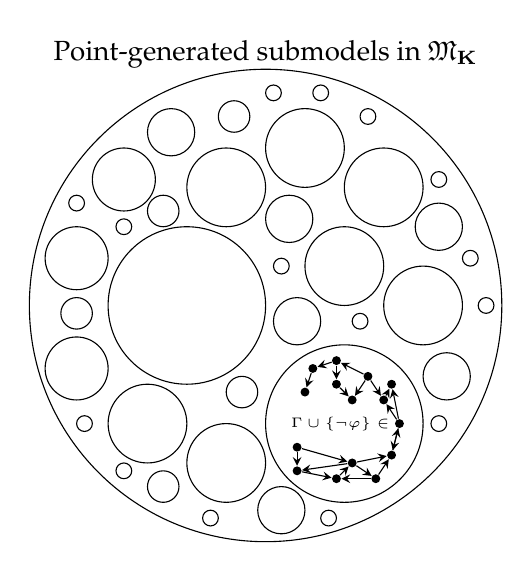
\begin{tikzpicture}[world/.style={inner sep=.4mm, fill=black, circle},>=stealth]

\draw  (0,0) ellipse (3 and 3);



\node[world](world) at (1.7,-1.5) {};

\node[anchor=east] at (world) {\tiny $\Gamma\cup \{\lnot \varphi \}\in$};

\pause

\node[world](a) at (0.9,-0.7) {};
\node[world](b) at (0.6,-0.8) {};
\node[world](c) at (1.3,-0.9) {};
\node[world](d) at (0.5,-1.1) {};
\node[world](e) at (0.9,-1) {};
\node[world](f) at (1.5,-1.2) {};
\node[world](g) at (1.6,-1) {};
\node[world](h) at (1.1,-1.2) {};
\node[world] (v6) at (1.6,-1.9) {};
\node[world] (v5) at (1.4,-2.2) {};
\node[world] (v3) at (0.9,-2.2) {};
\node[world] (v2) at (0.4,-2.1) {};
\node[world] (v1) at (0.4,-1.8) {};
\node[world] (v4) at (1.1,-2) {};
\begin{scope}[->]
\draw  (a) edge (e);
\draw  (c) edge (h);
\draw  (f) edge (g);
\draw  (c) edge (f);
\draw  (e) edge (h);
\draw  (c) edge (a);
\draw  (a) edge (b);
\draw  (b) edge (d);
\draw  (v1) edge (v2);
\draw  (v2) edge (v3);
\draw  (v3) edge (v4);
\draw  (v4) edge (v2);
\draw  (v4) edge (v5);
\draw  (v5) edge (v6);
\draw  (v4) edge (v6);
\draw  (v6) edge (world);
\draw  (v1) edge (v4);
\draw  (v5) edge (v3);
\draw  (world) edge (f);
\draw  (world) edge (g);
\draw  (world) edge (v6);
\end{scope}

\pause
\node(felirat) at (0,3.2) {\begin{tabular}{c}Point-generated  submodels in $\mathfrak M_{\mathbf K}$\end{tabular}};

\draw  (-1,0) ellipse (1 and 1);
\draw  (0.5,2) ellipse (0.5 and 0.5);
\draw  (1,0.5) ellipse (0.5 and 0.5);
\draw  (-0.5,-2) ellipse (0.5 and 0.5);
\draw  (1,-1.5) ellipse (1 and 1);
\draw  (2,0) ellipse (0.5 and 0.5);
\draw  (1.5,1.5) ellipse (0.5 and 0.5);
\draw  (-0.5,1.5) ellipse (0.5 and 0.5);
\draw  (-1.5,-1.5) ellipse (0.5 and 0.5);
\draw  (-2.4,-0.8) ellipse (0.4 and 0.4);
\draw  (-1.8,1.6) ellipse (0.4 and 0.4);
\draw  (-2.4,0.6) ellipse (0.4 and 0.4);
\draw  (0.4,-0.2) ellipse (0.3 and 0.3);
\draw  (0.3,1.1) ellipse (0.3 and 0.3);
\draw  (0.2,0.5) ellipse (0.1 and 0.1);
\draw  (-0.3,-1.1) ellipse (0.2 and 0.2);
\draw  (2.3,-0.9) ellipse (0.3 and 0.3);
\draw  (2.2,1) ellipse (0.3 and 0.3);
\draw  (-0.4,2.4) ellipse (0.2 and 0.2);
\draw  (-1.2,2.2) ellipse (0.3 and 0.3);
\draw  (-1.3,1.2) ellipse (0.2 and 0.2);
\draw  (0.2,-2.6) ellipse (0.3 and 0.3);
\draw  (-1.3,-2.3) ellipse (0.2 and 0.2);
\draw  (-2.4,-0.1) ellipse (0.2 and 0.2);
\draw  (1.2,-0.2) ellipse (0.1 and 0.1);
\draw  (2.6,0.6) ellipse (0.1 and 0.1);
\draw  (2.8,0) ellipse (0.1 and 0.1);
\draw  (2.2,-1.5) ellipse (0.1 and 0.1);
\draw  (1.3,2.4) ellipse (0.1 and 0.1);
\draw  (0.1,2.7) ellipse (0.1 and 0.1);
\draw  (0.7,2.7) ellipse (0.1 and 0.1);
\draw  (-2.4,1.3) ellipse (0.1 and 0.1);
\draw  (-1.8,1) ellipse (0.1 and 0.1);
\draw  (-2.3,-1.5) ellipse (0.1 and 0.1);
\draw  (-0.7,-2.7) ellipse (0.1 and 0.1);
\draw  (-1.8,-2.1) ellipse (0.1 and 0.1);
\draw  (0.8,-2.7) ellipse (0.1 and 0.1);
\draw  (2.2,1.6) ellipse (0.1 and 0.1);
\end{tikzpicture}}

\hazi{2}{1}{.7}{-5}{-4}{\begin{minipage}{3cm}Show that $\mathfrak M_{\mathbf{K}}$ is not connected! \end{minipage}}



\end{frame}

%%%%%%%%%%%%%%%%%%%%%%%%%%%%%%%%%%%%%%%%%%%%%%%%%%%%%%%%%%%%%%%%%%%%%%%%%%%%%%%%%%%%%%%%%%%%%%%%%%%5

\szakasz[Unraveling]{Unraveling}
\begin{frame}[t]
\frametitle{Logic of forests}
\footnotesize
\dzsa{Theorem} $\mathbf K+(4)$ is the logic of forests (too).
\bigskip

\dzsa{Idea:} We will transform the canonical model $\mathfrak M_{\mathbf K}$ into a forest $\mathrm{forest}(\mathfrak M_{\mathbf K})$ in a way that $\mathfrak M_{\mathbf K}$ will be a zig-zag image of $\mathrm{forest}(\mathfrak M_{\mathbf K})$. Therefore every formula will be satisfiable on a forest: on $\mathrm{forest}(\mathfrak M_{\mathbf K})$.

\bigskip

\[\mathrm{forest}(\mathfrak M_{\mathbf K})\defegy (\vec W_\mathbf K , \vec R_{\mathbf K}^t, \vec V_{\mathbf K})\]
where
\begin{itemize}
\item $\vec W_\mathbf K$ is the set of all finite paths in $W_\mathbf K$:
\[ \vec W_\mathbf K \defegy \{ \vec w \, :\, \textup{$\vec w$  is an $n$-tuple s.t. } w_1Rw_2R\dots Rw_n \} \]
\item $\vec R_{\mathbf K}^t$ is a transitive closure of $\vec w \vec R_\mathbf K \vec v$, where \\ $\vec w \vec R_\mathbf K \vec v$ iff $\vec v$ is a continuation of $\vec w$.
\[ \vec w \vec R_\mathbf K \vec v \defekv \existsin {u}{W_{\mathbf K}} \;  (\vec w, u) = \vec v \]
\item $\vec w \in \vec V_{\mathbf K}$ iff in the end of the past $\vec w$, $p$ is true ($\in V_{\mathbf K} (p)$).
\[ (w_1, \dots, w_n) \in \vec V_\mathbf K (p) \defekv w_n \in \vec V_{\mathbf K}(p) \]
\end{itemize}

Now the zigzag-morphism will be $h(w_1, \dots, w_n)= w_n$.

\pause

\hazi{2}{1}{.7}{4}{1}{\begin{minipage}{5cm}
Show that $\mathrm{forest}(\mathfrak M_{\mathbf K})$
is irreflexive, intransitive, antisymmetric.\end{minipage}}

\hazi{2}{1}{.7}{4}{0}{\begin{minipage}{5cm}
Show that $h$ is a surjective zigzag-morphism.\end{minipage}}

\end{frame}

%%%%%%%%%%%%%%%%%%%%%%%%%%%%%%%%%%%%%%%%%%%%%%%%%%%%%%%%%%%%%%%%%%%%%%%%%%%%%%%%%%%%%%%%%%%%%%%%%%%5

\begin{frame}
\frametitle{Examples}


\felirat{1.5}{1}{1}{0}{-.5}{
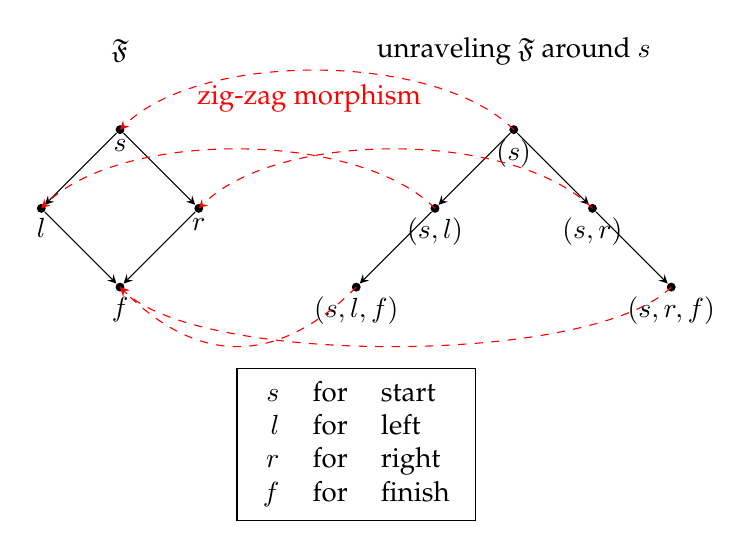
\begin{tikzpicture}[world/.style={inner sep=.4mm, fill=black, circle},>=stealth]


\node at (-2,2) {$\mathfrak F$};
\node at (3,2) {unraveling $\mathfrak F$ around $s$};
\node[draw=black] at (1,-3) {\begin{tabular}{rcl}
   $s$ &for& start
\\ $l$ &for& left
\\ $r$ &for& right
\\ $f$ &for& finish\end{tabular}};


\node[world] (v1) at (-2,1) {};
\node[world] (v2) at (-3,0) {};
\node[world] (v3) at (-1,0) {};
\node[world] (v4) at (-2,-1) {};

\begin{scope}[anchor=north]
\node at (v1){$s$};
\node at (v2){$l$};
\node at (v3){$r$};
\node at (v4){$f$};

\end{scope}

\begin{scope}[->]
\draw  (v1) edge (v2);
\draw  (v1) edge (v3);
\draw  (v2) edge (v4);
\draw  (v3) edge (v4);
\end{scope}

\pause

\node[world] (v5) at (3,1) {};
\node[world] (v6) at (2,0) {};
\node[world] (v8) at (4,0) {};
\node[world] (v7) at (1,-1) {};
\node[world] (v9) at (5,-1) {};

\begin{scope}[anchor=north]
\node at (v5){$(s)$};
\node at (v6){$(s,l)$};
\node at (v7){$(s,l,f)$};
\node at (v8){$(s,r)$};
\node at (v9){$(s,r,f)$};
\end{scope}


\begin{scope}[->]
\draw  (v5) edge (v6);
\draw  (v6) edge (v7);
\draw  (v5) edge (v8);
\draw  (v8) edge (v9);
\end{scope}


\pause

\node[red] at (0.4,1.4) {zig-zag morphism};

\begin{scope}[red, dashed, ->]
\draw (1,-1) .. controls (0,-2) and (-1,-2) .. (-2,-1);
\draw (5,-1) .. controls (4,-2) and (-1,-2) .. (-2,-1);
\draw (3,1) .. controls (2,2) and (-1,2) .. (-2,1);
\draw (4,0) .. controls (3,1) and (0,1) .. (-1,0);
\draw (2,0) .. controls (1,1) and (-2,1) .. (-3,0);
\end{scope}
\end{tikzpicture}}


\end{frame}

%%%%%%%%%%%%%%%%%%%%%%%%%%%%%%%%%%%%%%%%%%%%%%%%%%%%%%%%%%%%%%%%%%%%%%%%%%%%%%%%%%%%%%%%%%%%%%%%%%%5

\begin{frame}
\frametitle{Examples}


\felirat{1.5}{1}{1}{0}{-.65}{


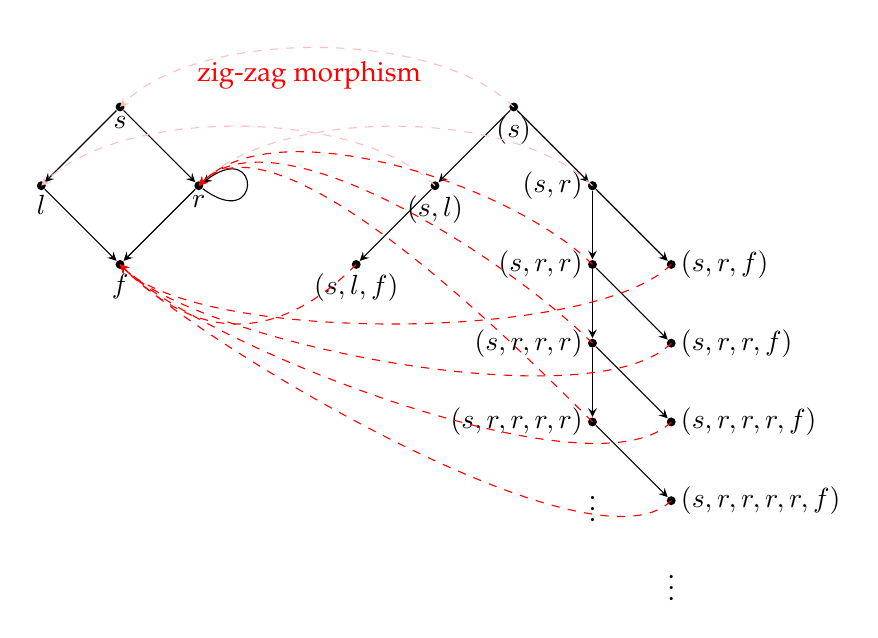
\begin{tikzpicture}[world/.style={inner sep=.4mm, fill=black, circle},>=stealth]

\node[world] (v1) at (-2,1) {};
\node[world] (v2) at (-3,0) {};
\node[world] (v3) at (-1,0) {};
\node[world] (v4) at (-2,-1) {};


\begin{scope}[anchor=north]
\node at (v1){$s$};
\node at (v2){$l$};
\node at (v3){$r$};
\node at (v4){$f$};
\end{scope}

\begin{scope}[->]
\draw  (v1) edge (v2);
\draw  (v1) edge (v3);
\draw  (v2) edge (v4);
\draw  (v3) edge (v4);
\end{scope}


\pause
\draw[->]  (v3) .. controls (-0.2,-0.6) and (-0.2,0.6) .. (v3);
\pause

\node[world] (v5) at (3,1) {};
\node[world] (v6) at (2,0) {};
\node[world] (v8) at (4,0) {};
\node[world] (v7) at (1,-1) {};
\node[world] (v9) at (5,-1) {};


\begin{scope}[anchor=north]
\node at (v5){$(s)$};
\node at (v6){$(s,l)$};
\node at (v7){$(s,l,f)$};
\end{scope}

\begin{scope}[anchor=east]
\node at (v8){$(s,r)$};
\end{scope}

\begin{scope}[anchor=west]
\node at (v9){$(s,r,f)$};
\end{scope}



\begin{scope}[->]
\draw  (v5) edge (v6);
\draw  (v6) edge (v7);
\draw  (v5) edge (v8);
\draw  (v8) edge (v9);
\end{scope}

\pause

\node[world] (v10) at (4,0) {};
\node[world] (v11) at (4,-1) {};
\node[world] (v12) at (5,-2) {};
\node[world] (v13) at (4,-2) {};
\node[world] (v14) at (5,-3) {};
\node[world] (v15) at (4,-3) {};
\node[world] (v16) at (5,-4) {};

\begin{scope}[anchor=east]
\node at (v11){$(s,r,r)$};
\node at (v13){$(s,r,r,r)$};
\node at (v15){$(s,r,r,r,r)$};
\end{scope}

\begin{scope}[anchor=west]
\node at (v12){$(s,r,r,f)$};
\node at (v14){$(s,r,r,r,f)$};
\node at (v16){$(s,r,r,r,r,f)$};
\end{scope}

\begin{scope}[->]
\draw  (v10) edge (v11);
\draw  (v11) edge (v12);
\draw  (v11) edge (v13);
\draw  (v13) edge (v14);
\draw  (v13) edge (v15);
\draw  (v15) edge (v16);
\end{scope}

\node at (4,-4) {$\vdots$};
\node at (5,-5) {$\vdots$};

\pause

\node[red] at (0.4,1.4) {zig-zag morphism};

\begin{scope}[pink, dashed, ->]
\draw (3,1) .. controls (2,2) and (-1,2) .. (-2,1);
\draw (4,0) node (v10) {} .. controls (3,1) and (0,1) .. (-1,0);
\draw (2,0) .. controls (1,1) and (-2,1) .. (-3,0);
\end{scope}

\pause

\begin{scope}[red, dashed, ->]
\draw (1,-1) .. controls (0,-2) and (-1,-2) .. (-2,-1);
\draw (5,-1) .. controls (4,-2) and (-1,-2) .. (-2,-1);
\draw (5,-2) .. controls (4,-3) and (-1,-2) .. (-2,-1);
\draw (5,-3) .. controls (4,-4) and (-1,-2) .. (-2,-1);
\draw (5,-4) .. controls (4,-5) and (-1,-2) .. (-2,-1);
\draw (4,-1) .. controls (3,0) and (0,1) .. (-1,0);
\draw (4,-2) .. controls (3,-1) and (0,1) .. (-1,0);
\draw (4,-3) .. controls (3,-2) and (0,1) .. (-1,0);
\end{scope}


\end{tikzpicture}
}


\end{frame}


%%%%%%%%%%%%%%%%%%%%%%%%%%%%%%%%%%%%%%%%%%%%%%%%%%%%%%%%%%%%%%%%%%%%%%%%%%%%%%%%%%%%%%%%%%%%%%%%%%%5



\begin{frame}
\frametitle{Examples}


\hazi{1.5}{1}{1}{0}{-.65}{\raisebox{1cm}{Unravel this around $w$:}\qquad
$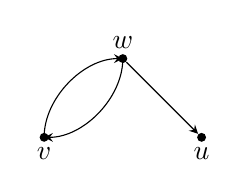
\begin{tikzpicture}[world/.style={inner sep=.4mm, fill=black, circle},>=stealth]

\node[world] (v1) at (-2,1) {};
\node[world] (v2) at (-3,0) {};
\node[world] (v3) at (-1,0) {};

\begin{scope}[anchor=north]
\node at (v2){$v$};
\end{scope}

\begin{scope}[anchor=south]
\node at (v1){$w$};
\end{scope}

\begin{scope}[anchor=north]
\node at (v3){$u$};
\end{scope}

\begin{scope}[->]
\draw (-3,0) .. controls (-3,0.5) and (-2.5,1) .. (-2,1);
\draw (-2,1) .. controls (-2,0.5) and (-2.5,0) .. (-3,0);
\draw  (v1) edge (v3);
\end{scope}
\end{tikzpicture}
$}


\end{frame}

%%%%%%%%%%%%%%%%%%%%%%%%%%%%%%%%%%%%%%%%%%%%%%%%%%%%%%%%%%%%%%%%%%%%%%%%%%%%%%%%%%%%%%%%%%%%%%%%%%%5



\begin{frame}[t]
\frametitle{Logic of transitive forests}
\footnotesize
\dzsa{Corollary} $\mathbf K+(4)$ is the logic of \textbf{trees} (too).
\bigskip

\pause

\hazi{2}{1}{.7}{4}{-2}{\begin{minipage}{5cm}
Prove that statement\end{minipage}}

\end{frame}

%%%%%%%%%%%%%%%%%%%%%%%%%%%%%%%%%%%%%%%%%%%%%%%%%%%%%%%%%%%%%%%%%%%%%%%%%%%%%%%%%%%%%%%%%%%%%%%%%%%5

\szakasz[Bulldozing]{Bulldozing}

\begin{frame}
\frametitle{Examples}


\felirat{1.5}{1}{1}{0}{-.65}{
\begin{tikzpicture}[world/.style={inner sep=.4mm, fill=black, circle},>=stealth]

\node  (v1) at (-5,1) {};
\node[world]  (v2) at (-4,1) {};
\draw[->]  (v1) edge (v2);

\pause

\node[world]  (v3) at (-3,1) {};
\draw[->]  (v2) edge (v3);

\pause

\node[world]  (v4) at (-2,1) {};
\draw[->]  (v3) edge (v4);

\pause

\node(kp) at (0,1) {};
\foreach \i in {30,60,...,360}{\node(vilag\i)[world] at ([shift=(\i: 1cm)]kp){};}
\foreach \i in {30,60,...,360}{\foreach \j in {30,60,...,\i}{\draw (vilag\j)--(vilag\i);}}
\foreach \i in {30,60,...,360}{\draw[->] (vilag\i) .. controls ([shift=(\i+-45:.5)]vilag\i) and  ([shift=(\i + 45:.5)]vilag\i) .. (vilag\i);
}

\draw[->]  (v4) edge (vilag180);


\pause

\node[world] (v5) at (2,1) {};
\draw[->]  (vilag360) edge (v5);

\node[world] (v6) at (3,1) {};
\draw[->]  (v5) edge (v6);

\node[world] (v7) at (4,1) {};
\draw[->]  (v6) edge (v7);

\node (v8) at (5,1) {};
\draw[->]  (v7) edge (v8);

\pause

\node at (-3,2){
\includegraphics[scale=.3]{bulldozer.png}};

\pause

\node at (-3,0.25){\tiny\begin{minipage}{3cm} 1. Find the cluster \\ (i.e., cycle or largest universally related subframe)\end{minipage}};

\pause

\node at (3,2){\tiny\begin{minipage}{2cm} 2. Choose a path that roams the cluster\end{minipage}};

\draw[red, ultra thick,->] (vilag180)
->(vilag30)
->(vilag90)
->(vilag60)
->(vilag210)
->(vilag270)
->(vilag300)
->(vilag150)
->(vilag120)
->(vilag240)
->(vilag330)
->(vilag360);


\pause

\node at (-4,-1){\tiny\begin{minipage}{1.5cm} 3. Copy that path $\mathbb Z$-many times\end{minipage}};

\foreach \j in {-3,-2, ..., 3}{\node at (-3,-2-.5*\j){\j};
\foreach \i in {1,2,...,12}{\node(\j egy\i)[world] at (-3+.5*\i,-2-.5*\j){};}}

\foreach \j in {-3,-2, ..., 3}{
\foreach \i in {1,2,...,11}{
\pgfmathtruncatemacro{\suci}{\i+1}
\draw[red,->](\j egy\i)--(\j egy\suci);}}


\pause

\node at (-4,-3){\tiny\begin{minipage}{1.5cm} 4. Link them together into a line\end{minipage}};


\foreach \j in {-3,-2, ..., 2}{
\pgfmathtruncatemacro{\sucj}{\j+1}
\draw[red,->](\j egy12)edge[in=25, out=-25](\sucj egy1);}


\pause

\node at (4.5,-2){\tiny\begin{minipage}{1cm} 5. Replace the cluster with that infinite (line) route\end{minipage}};


\end{tikzpicture}
}


\end{frame}

%%%%%%%%%%%%%%%%%%%%%%%%%%%%%%%%%%%%%%%%%%%%%%%%%%%%%%%%%%%%%%%%%%%%%%%%%%%%%%%%%%%%%%%%%%%%%%%%%%%5

\begin{frame}
\frametitle{Bulldozing}

\dzsa{Theorem} Every K4.3 model is a zig-zag image of its bulldozed model.

\bigskip

\dzsa{Proposition} Every bulldozed model of a K4.3 model is acyclic (i.e., irreflexive and is free from any equivalence related subframes).

\bigskip

\dzsa{Corollary} Every point-generated subframe of a bulldozed model of a K4.3 model is trichotomic.

\bigskip

\dzsa{Corollary} K4.3 is the temporal logic of flow of times (= STO's = strict total orders).

\hazi{1.5}{1}{1}{0}{-3.25}{\begin{minipage}{7cm}\textbf{Workshop topic:} Formalize the idea of bulldozing and prove that theorem above. \\ (Source: Blackburn--de Rijke--Venema: Thm 4.56.\\ though I think it is easier to develop this formalism by yourself -- it is quite hard to read a formalism like that unless you were the one who wrote it.)\end{minipage}}

\end{frame}

%%%%%%%%%%%%%%%%%%%%%%%%%%%%%%%%%%%%%%%%%%%%%%%%%%%%%%%%%%%%%%%%%%%%%%%%%%%%%%%%%%%%%%%%%%%%%%%%%%%5

\end{document}
